\documentclass[11pt]{article}   
\usepackage{times, latexsym, amsmath, marginnote, epsfig, amsfonts, graphicx, paralist, subfig, rotating, color, booktabs, multirow,url, float}  % , natbib
\usepackage[linesnumbered,lined,boxed,commentsnumbered]{algorithm2e}
\usepackage[margin=1in]{geometry}
%\usepackage{tex-gyre}
\usepackage{mathrsfs}
%\usepackage{subcaption}
\usepackage{tikz}
\usetikzlibrary{shapes.geometric, arrows}

\tikzstyle{standard} = [rectangle, rounded corners, minimum width=1.5cm, minimum height=2cm,text width=2.5 cm, text centered, draw=black, fill=black!5]
\tikzstyle{io} = [trapezium, trapezium left angle=70, trapezium right angle=110, minimum width=3cm, minimum height=1cm, text centered, draw=black, fill=blue!30]
\tikzstyle{process} = [rectangle, minimum width=3cm, minimum height=1cm, text centered, text width=3cm, draw=black, fill=orange!30]
\tikzstyle{decision} = [diamond, minimum width=3cm, minimum height=1cm, text centered, draw=black, fill=green!30]
\tikzstyle{arrow} = [thick,->,>=stealth]

\SetKwInOut{Parameter}{parameter}
\renewcommand{\familydefault}{ptm}  
\setlength{\parindent}{0cm}
\setlength{\parskip}{1em}%
\newcommand{\HRule}{\rule{\linewidth}{0.5mm}} 
\DeclareMathOperator*{\argmin}{arg\,min}
\DeclareMathOperator*{\argmax}{arg\,max}


	% =======================================================================
	\begin{document}
	% =======================================================================
	\title{Early classification of spatio-temporal events using time-varying models}
	\author{Sevvandi Kandanaarachchi, Rob J. Hyndman, Kate Smith-Miles}
	\maketitle
	\abstract{This paper investigates early event classification in spatio-temporal data streams.  We propose a framework for early classification that considers the relationship between the features of an event and their age. The framework incorporates an event extraction algorithm as well as two early event classification algorithms, which use a series of logistic regression classifiers with penalty terms and state space models.  We use this framework on synthetic and real-world applications and demonstrate its reliability and broad applicability. The algorithms are available in the R package {\it eventstream}, and other code in the supplementary material.   }
	
	%% Outline of paper
	%% Introduction
	%% 		- Small introduction to data-streams and interesting topics
	%%		- Events that change over time
	%%		- Real world example
	%%		- Why standard classifiers may be not enough
	%% 		- Example - RF and event classifier
	%%		- General workflow
	%%			 Data stream -> Pre-processing -> Event extraction -> Features -> Event classification
	%%		- Main focus is on classification
	%% 		- Two methods - static and updating
	%%		- Mention eventstream package
	%% Event extraction
	%%		- threshold and cluster
	%% Event classification
	%%		- Cyclic logisitic regression (with penalty)
	%%		- Cascaded DMA
	%% Applications
	%%		- Synthetic data
	%% 			- Comparison with glm
	%%		- Fibre optic data - event classification
	%% 			- Comparison with glm
	%% 		- NO2 data - event extraction

	%% Future work and Conclusions
	



	% =======================================================================
	\section{Introduction}
	% =======================================================================
	
	Early detection and classification of emerging events - however they are defined - in data streams is an important challenge in our data-rich world. Events in data streams may stem from different applications such as social media, Internet of Things, video surveillance, epidemiology and wireless sensors to name a few. Often these applications are associated with different disciplines, where discipline-specific techniques existed before data streaming became a common phenomenon. Due to this reason, it is customary to see existing techniques extended to a streaming context, giving rise to little consensus on associated terminology across disciplines.  
	
	On one hand, similar terms are used to describe different phenomena. This is called the synonym problem \cite{zhou2014spatiotemporal}. On the other hand, different terms are used to describe similar phenomena, which is called the homonym problem \cite{zhou2014spatiotemporal}. This makes it difficult to objectively compare results and methods across disciplines. For example, the term ``event detection'' is used in video surveillance and video applications \cite{adam2008robust, ke2005efficient, medioni2001event}, social media \cite{weng2011event, li2012tedas, abdelhaq2013eventweet}, broadcast news stories \cite{allan1998line, li2005probabilistic} and wireless sensor networks \cite{yin2009spatio, mao2015online}. However, it is difficult to apply an event detection method used in one application to another domain as many contextual properties depend on the problem domain, resulting in a proliferation of custom-made algorithms. As a result event detection has become a discipline-specific study with little overlap between different research problems. 
	
	Similarly spatio-temporal event detection, which is a popular sub-topic, has emerged from different applications such as river sensor networks \cite{mao2015online}, traffic data \cite{souto2016event}, wireless sensor networks \cite{mousavi2013spatio}, social networks \cite{cheng2014event} and epidemiology \cite{gomide2011dengue}. While spatio-temporal event detection is  studied reasonably well, early classification of spatio-temporal events has not received much attention. Mostly standard classification techniques are used on detected events while the focus has been on event detection \cite{kang2014detecting}. 
	
	%OK, so you are describing a situation where the feature vector can't really be computed accurately until the event is finished (so we can know it's shape etc.) but at earler times we have an incomplete/partial observation, and we want to know if we can use this to do early classifation of events (assuming that we have already been successful in early detection of events?)
	
	We are interested in events that start, develop for some time and stop at a certain time. Along with the event features, we use the ``age'' to describe these events.  We note that the age and time of events are different quantities. The age of an event is the time duration for which it has been growing, i.e. the difference between the current time and the start time of the event, where as time refers to the current time. 
	
	For events with age-varying behaviour standard classification techniques may not be suitable, if early detection is important. This is because the event features may change as the event progresses, such that an accurate feature vector can only be computed after the event is finished. However, for applications where early classification is important, this is not satisfactory as one cannot wait until the event  finishes to classify it.  While the event is still progressing, we have access to incomplete/partial information,  giving rise to a premature/incomplete feature vector. Our focus is on classifying events using this premature feature vector.  To do this we incorporate age-varying coefficients in our model similar to the varying coefficients models \cite{hastie1993varying}. A linear model with age-varying coefficients is given by Equation \eqref{eq:Int1}:
	
	\begin{equation}\label{eq:Int1}
	y_t = a_0(t)  + a_1(t) x_1(t) + \ldots + a_b(t)x_b(t) + \epsilon_t \, , 
	\end{equation} 
	\noindent
	where $y_t$ is the output at age $t$, $a_i(t)$ are the age-varying coefficients and $x_i(t)$ are the attributes of the event at age $t$. A logistic model with age-varying coefficients is given by Equations \eqref{eq:Int1} and  \eqref{eq:Int2}:
	
	\begin{equation}\label{eq:Int2}
	z_t = \frac{e^{y_t}}{1 + e^{y_t}} \, ,
	\end{equation} 
	\noindent
	where $z_t$ is the probability, an event of age $t$ belongs to a given class in the two class scenario. As an event develops, the features $x_i(t)$ change with the age of the event, while keeping the class label constant. Thus, it is clear that the coefficients $a_i(t)$ need to change with the age of the event. 

	At this point, we note that concept drift \cite{widmer1996learning, tsymbal2004problem,klinkenberg2000detecting,gama2014survey} or non-stationarity of data streams \cite{hulten2001mining, gama2010knowledge, gaber2005mining} is different from  age-varying events. As we will show in Section \ref{subsec:Synthetic}, age-varying events can occur in stationary data streams or data streams without any concept drift. This is because age-varying behaviour is change within the event as opposed to a change in the data stream. Even though non-stationarity and time-varying models has been studied in different contexts \cite{harvey1989time, wang1998cluster, hoover1998nonparametric}, they have not been explored for premature event classification to the best of our knowledge. 
	
	 %may last  time-dependent class boundary is not encapsulated in standard classifiers. 
	% Our focus is on early classification of time dependent events. Specifically, early classification of spatio-temporal events with contiguous spatial dimensions.  
	%We note that age and time are different quantities. The age of an event is the time duration for which it has been growing, i.e. the difference between the current time and the birth time of the event, where as time refers to the current time.  We investigate time-dependent models for spatio-temporal events that change with event-age. 
	
	We explore early event classification using two approaches that are based on different principles: \begin{inparaenum} \item logistic regression, and \item  state-space models.  \end{inparaenum} These two approaches complement each other as logistic regression by itself is a static model more suited for stationary distributions, and a state space model coupled with a Kalman filter can update easily, which is advantageous for non-stationary data distributions. On the other hand, logistic regression may give better results than state space models for a stable data distribution.   
	
	Our proposed framework, depicted in Figure \ref{fig:1}  can be used in real-world applications that give rise to spatio-temporal events with contiguous spatial dimensions. Typically pre-processing is also a common step done before event extraction. However we do not focus on pre-processing data as techniques differ depending on the application.  As event extraction is needed before classification  we also propose a simple method for event extraction. We make this work available in the R package {\it eventstream}. 
	
	\begin{figure}[H]
	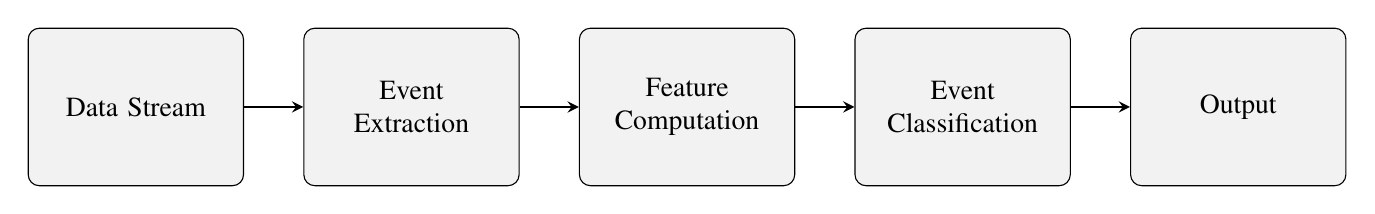
\begin{tikzpicture}[node distance=2cm]
	
	\node (start) [standard] {Data Stream};
	\node (extract) [standard, right of=start, xshift=1.5cm] {Event \\ Extraction};
	\node (features) [standard, right of=extract, xshift=1.5cm] {Feature \\ Computation};
	\node (classify) [standard, right of=features, xshift=1.5cm] {Event \\ Classification};
	\node (output) [standard, right of=classify, xshift=1.5cm] {Output};
			
	\draw [arrow] (start) -- (extract);
	\draw [arrow] (extract) -- (features);
	\draw [arrow] (features) -- (classify);
	\draw [arrow] (classify) -- (output);

	\end{tikzpicture}
	\caption{\footnotesize Framework for event extraction and classification for spatio-temporal data}
	\label{fig:1}
	\end{figure}
	
	Figure \ref{fig:Real_World_Data} gives the heatmap of a real word dataset we use for early event classification. This dataset is produced from a fibre optic  cable. A pulse is periodically sent through the cable and this results in a data matrix where each horizontal row gives the strength of the signal at a fixed location $x_0$, and each vertical column gives the strength of the signal along the cable at a fixed time $t_0$.  In this dataset the yellow parts represent high intensity values and the blue parts represent low intensity values. 
	
	\begin{figure}[H]
	\centering
	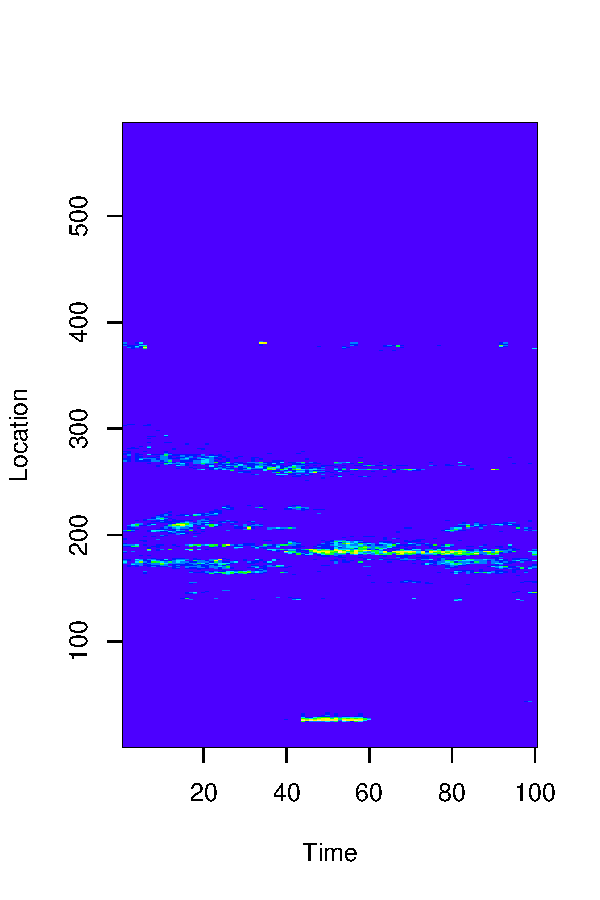
\includegraphics{./Graphics/Real_World.pdf}  % Real_World_Ex2.pdf
	\caption{\footnotesize Real world dataset}
	\label{fig:Real_World_Data}
	\end{figure}
	
	Fibre optic sensor cables are used in many applications including optical communications, detecting undersea cable faults \cite{jiang2009technological}, detecting oil leakages \cite{nikles2004leakage}, detecting intruders on secured premises \cite{griffiths1995developments}, monitoring health of infra-structure such as bridges and pipe-lines \cite{li2004recent}, to name a few. Due to its sensitivity, fibre optic cables are also prone to noise. In the dataset in Figure \ref{fig:Real_World_Data}, events are the yellow and yellow-blue parts that stand out. In a setting where early classification is  important, we need to classify these events quickly, preferably while they are still ongoing. In the dataset shown in Figure \ref{fig:Real_World_Data} there are two classes of events: classes A and B. The event approximately at location 30 between the time interval  45 to 60 is of class A while other events that appear between locations 150 and 400  are of class B. Due to the commercially sensitive nature of the dataset, we refrain from giving details about the actual application. However, one can associate events in each of the applications listed above as either belonging to class A or B. For example a cable lying on the sea bed can produce spatio-temporal events that are either cable faults, or non-fault events due to the activity in the ocean. 
	
	
	We investigate early classification of spatio-temporal events using the framework in Figure \ref{fig:1}. The remainder of the paper is organized as follows: Section \ref{sec:EventExtract} discusses event extraction and feature computation. Section \ref{sec:Notation}  introduces the notation for classification of developing-events. In Sections \ref{sec:ExtendedClassifier} and  \ref{sec:CascadedDLM} we introduce the developing-events classifier and the cascaded non-Gaussian state space models respectively. %In Section \ref{sec:Experiments}  we discuss the synthetic datasets, and the results of the two early detection methods. 
	In Section \ref{sec:Experiments} we discuss results of our framework using synthetic data and two real-world applications. The first  application is associated with the dataset in Figure \ref{fig:Real_World_Data} and the second application is on Nitrogen dioxide $(\text{NO}_2)$ data from NASA's  NEO \cite{OMINO2} website. Finally in Section \ref{sec:Conclusions} we present our conclusions and discuss future work.  
	
		
	% =======================================================================
	% =======================================================================
	\section{Event extraction and feature computation} \label{sec:EventExtract}
	% =======================================================================
	
	\subsection{Event extraction}
	 We extract events from data streams of 2 or 3 dimensions, i.e. 1 spatial $ \times $ 1 time dimension or 2 spatial $ \times $ 1 time dimension.  We employ a simple method for event extraction as this is not our primary research goal.  Event extraction is done using DBSCAN \cite{ester1996density}, which is a density based clustering algorithm. Our event extraction algorithm is explained in Algorithm \ref{algo:events_extraction}.
	 
	 \DontPrintSemicolon
	 \begin{algorithm}[!ht]
	 	\footnotesize
	 	\SetKwInOut{Input}{input}
	 	\SetKwInOut{Output}{output}
	 	\Input{a 2 or 3-dimensional array $A_{n\times m}$ or $A_{n\times m \times k}$ , and parameters $\alpha$, $\epsilon$ and {\it minPts}. }
	 	\Output{events: $A|_S \subset A$  and the event ids for each $s_{ij} \in A|_S$ (or $s_{ijk}$ if $A$ is 3-dimensional. }
	 	Let $a_{ij}$ be the signal value at $(i, j)$ position of $A$, if $A$ is 2-dimensional and $a_{ijk}$ be the signal value at $(i, j, k)$ position of $A$ if $A$ is  $3-$ dimensional. \\
	 	Let $q$ denote the $\alpha^{\text{th}}$ percentile of the signal values of $A$. \\
	 	$S = \{ (i,j) \hspace{2mm} | \hspace{2mm} a_{ij} > q  \} $ for 2-dimensional $A$ and 
	 	$S = \{ (i,j, k) \hspace{2mm} | \hspace{2mm} a_{ijk} > q  \} $ for 3-dimensional $A$. \\
	 	$ B = A|_S$, i.e. signal values of $A$ in $S$ locations. \\
	 	Using DBSCAN cluster B using $\epsilon$ and {\it minPts}. \\
	 	This clustering gives each $s \in A|_S$ a cluster id. \\
	  	%Convert $A$ to a mesh-grid format $B$, i.e. $B$ contains 2D/3D grid coordinates and the value of each cell of $A$.  \;
	    %Of the cell values, get the positions and values of $B$ greater than $\alpha^{\text{th}}$ percentile. \;
	    %Using DBSCAN cluster the chosen cells using $\epsilon$ and {\it minPts}. \;
	 	
	 	Consider each cluster as a event. \, 
	 	\caption{\footnotesize Extract events from a dataset or window}
	 	\label{algo:events_extraction}
	 \end{algorithm}
	 
	 A synthetic dataset generated from the package {\it eventstream} and the events extracted using Algorithm \ref{algo:events_extraction} are shown in Figure \ref{fig:blobs_A_B}. 
	 
	 \begin{figure}[H]
	 	\centering
	 	\subfloat[][]{
	 		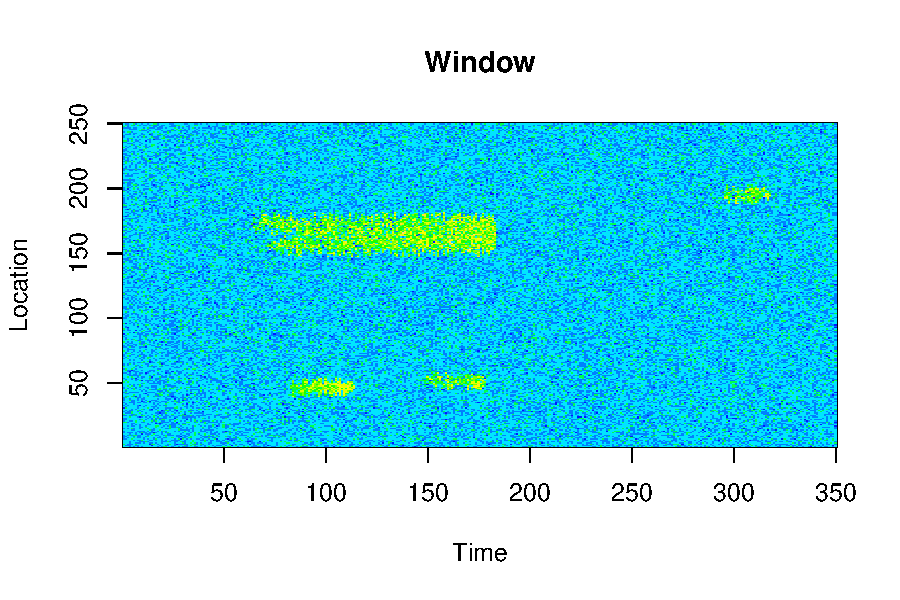
\includegraphics[scale=0.5]{./Graphics/gen_data.pdf} % 3_B_Blobs.pdf ./Graphics/Extracted_Blobs_A_file.pdf
	 		\label{fig:Class_A_1}
	 	}%
	 	\subfloat[][]{
	 		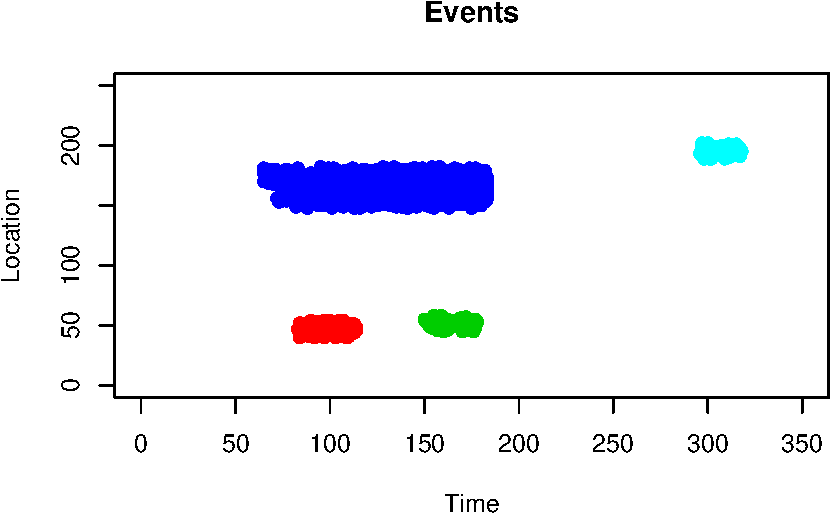
\includegraphics[scale=0.5]{./Graphics/events_extracted.pdf}  % Extracted_Blobs_Class_B_file.pdf
	 		\label{fig:Class_B_1}
	 	}
	 	\caption{\footnotesize A synthetic dataset from {\it eventstream} and the events extracted from it.} 
	 	\label{fig:blobs_A_B}
	 \end{figure}
	 
	 \subsection{Features}\label{sec:Featurelist}
	 As we work with a data stream, we use a moving window model in our experiments. We extract events from data in the current window and compute features for these events. The feature set comprises of some basic features such as length and width of each event, and some other features that compute the intensity of each event relative to the background. ``Relative to the background'' features  are motivated from the real world application (see Figure \ref{fig:1}) and are only computed for two-dimensional data streams.  
	 
	 To compute the ``relative to the background'' features  we use smoothing splines. Using a small portion from the beginning of each window we compute the mean, median, IQR and standard deviation for each location. Using these values at each location, we compute four smoothing splines. The objective is to have the background mean, median, IQR and standard deviation pixel value for each location.  The median and IQR splines from a small window in Figure \ref{fig:Im_Splines} are shown in Figures \ref{fig:Spline_Median} and \ref{fig:Spline_IQR}. %This enables the computation of event strength or intensity relative to the background.
	 
	\begin{figure}[H]
		 	\centering
		\subfloat[][]{
			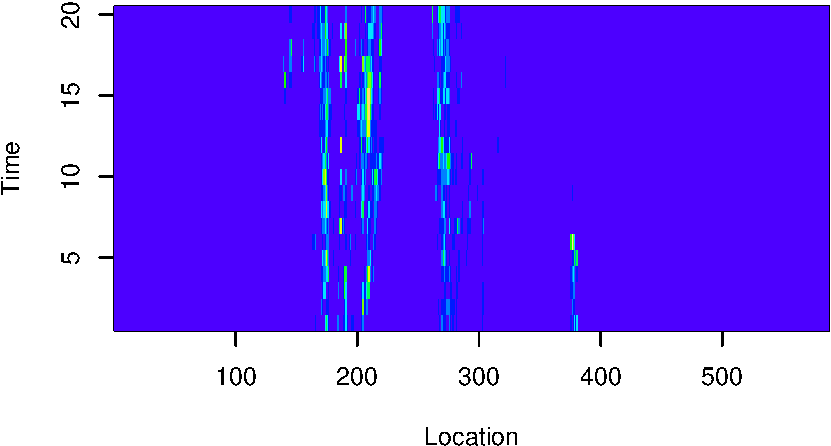
\includegraphics[scale=0.35]{./Graphics/Image_for_Splines.pdf} % 
			\label{fig:Im_Splines}
		}%
		\subfloat[][]{
			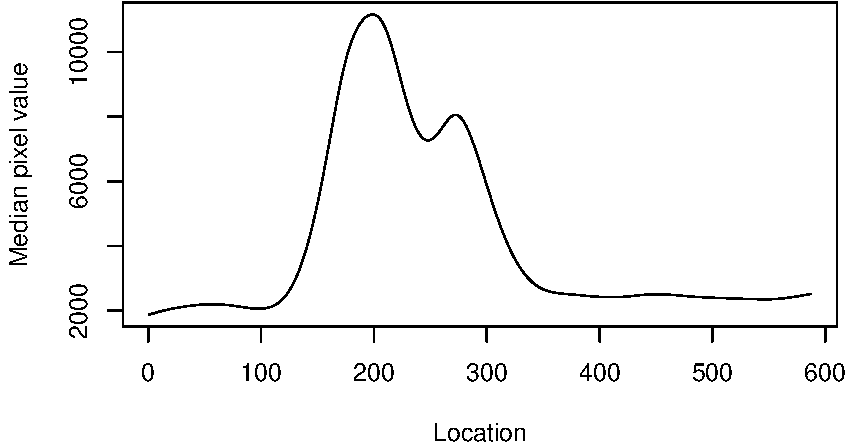
\includegraphics[scale=0.35]{./Graphics/Spline_Median.pdf}
			\label{fig:Spline_Median}
		}
		\subfloat[][]{
		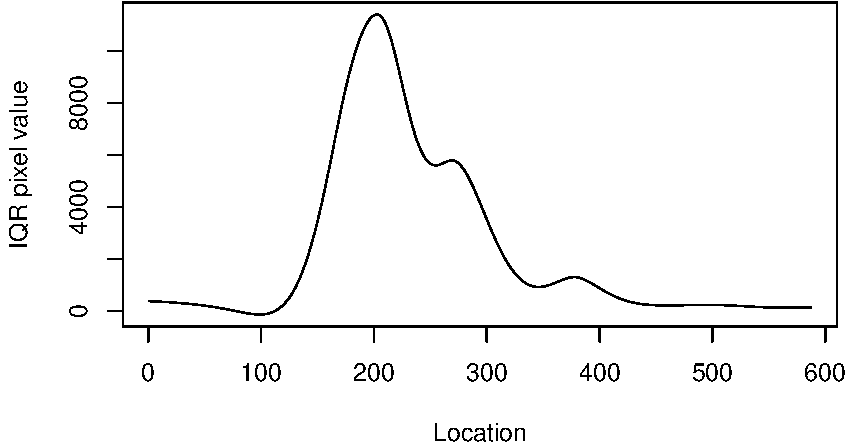
\includegraphics[scale=0.35]{./Graphics/Spline_IQR.pdf}
		\label{fig:Spline_IQR}
		}
		\caption{\footnotesize The initial portion of a window and the resulting median and IQR splines.} 
		\label{fig:splines}
	\end{figure}		
	 
	 
	 For two-dimensional events we compute the following features:	 
	  \begin{enumerate}
	 	\item Number of cells/pixels in event
	 	\item Length of event
	 	\item Width of event
	 	\item Length to width ratio of event
	 	\item Centroid \\
	 	The centroid is used to compute other features which are relative to the event. It is not used in  event classification.
	 	\item Sum of cell-values of cells in event
	 	\item Mean cell-value of event
	 	\item Standard deviation of cell-values of event
	 	\item Slope of the fitted line $l$ \\
	 	The average pixel value at each time of the event is computed and a line  $l$  is fitted to the average values. The slope of the fitted line $l$ is a feature of interest . 
	 	\item Linear and quadratic coefficients of a fitted parabola $p$ \\
	 	The average pixel value at each time of the event is computed and a parabola  $p$  is fitted to the average values. The linear and quadratic coefficients of the fitted parabola $p$ are features of interest. 
	 	\item $n$ standard deviations from the mean \\
	 	The proportion of event pixels that has values greater than $n$ global standard deviations from the global mean for $n \in \{2, 3, 4\}$. 
	 	\item $n$ local IQR from local median \\
	 	%We use a small portion from the beginning of each window to compute smoothing splines which are indicative of the level of activity or noise for each location. Four smoothing splines are computed using the horizontal row means, medians, IQR values and standard deviation values. For example from the initial slice of data, the IQR is computed for each horizontal row and a smoothing spline is fitted to these IQR values giving the IQR spline. 
	 	The value of the median smoothing spline at each event centroid is used as the local median for that event. Similarly, the value of the IQR smoothing spline at each event centroid is used as the local IQR for that event. This feature gives the proportion of event pixels/cells that has values greater than $n$ local IQRs from the local median for $n \in \{ 5, \ldots, 8 \} $
	 %	\item $n$ standard deviation from spline mean \\
	 %	Similar to the previous feature, this feature gives the proportion of event pixels/cells that has values greater than $n$ local means from the local standard deviation for $n \in \{2, \ldots, 7 \}$.
	 	\item Local IQRs from local median \\
	 	Let us denote the $75^\text{th}$ percentile of the event pixel value by $x$. This feature gives the number of local IQRs that $x$ is greater than the local median. Both local IQR and local median are computed using splines described above. 
	 	\item Local standard deviation from local mean \\
	 	Similar to the previous feature, our $x$ is the $80^\text{th}$ percentile of the event pixel value. Here we compute the number of local standard deviations $x$ is greater than the local mean.
	 \end{enumerate}
	 
	For three-dimensional data streams we compute a subset of the above features. In particular, we compute features  1 - 8 from the above list and an equivalent of feature 14 using the global standard deviation and the global mean. Having extracted events and computed features, we are ready to explore the challenges in classifying developing events. 
	
	 
	% =======================================================================
	% =======================================================================
	\section{Notation for developing-events classifier} \label{sec:Notation}
	% =======================================================================
	In the classical setting, a classification problem comprises of observations $\left(\mathbf{x}_i, y_i \right)$ for $i \in 1\ldots N$ where $\mathbf{x}_i \in \mathbb{R}^b$ is the attribute vector of the $i^{\text{th}}$ observation and $y_i$ is its class label. The task of the classifier is to learn the class boundary by using the given set of observations. Then for any new observation $\mathbf{x}_j$ the classifier can predict its class label using the already learned class boundaries. Let us call this a {\textbf{standard classifier}}. 
	
	Standard classifiers have been widely popular in diverse fields of study and practice. However, they are not without limitations. One of the limitations is that once a classifier is trained, it has fixed class boundaries. If the new data is different from the data learned by the classifier, the output of the classifier is of little use. This is specially the case in data-streaming scenarios, where data distributions are non-stationary. It is also referred to as concept drift. It is necessary for a classifier to re-adjust its class boundaries when faced with concept drift. The literature on adapting or evolving classifiers is significant \cite{duchi2011adaptive, dabbagh2005online, frey1991letter, giacinto1997adaptive, nishida2005ace,alippi2008just, alippi2008just2}. Let us call these classifiers {\bf{evolving classifiers}}.  
 
 
	Now, consider the case when a new observation is not made available at once but gradually. By gradually we mean that we get partial information of the new observation and the amount of partial information increases with time. This is specially the case for events described in Section \ref{sec:EventExtract}.  Let $\mathbf{x}_j$ be  a new observation, and say it becomes available partially as the following finite sequence of partial observations $\left \{\mathbf{p}^j_{t_1},\mathbf{p}^j_{t_2}, \mathbf{p}^j_{t_3}, \ldots,  \mathbf{p}^j_{t_n} \right \}$. Here the partial observation of $\mathbf{x}_j$ of age $t_k$ is denoted by $\mathbf{p}^j_{t_k}$ and   $\mathbf{p}^j_{t_n} = \mathbf{x}_j$ with $t_1 < t_2 < \ldots < t_n$.  Here we differentiate between the time and the age of a partial observation. A partial observation that begins at time $t =t_1$ has age $0$ at time $t_1$, and at time $t = t_2$ has age $ t_2 - t_1$. 
	
	
	
	We consider the question ``how can we classify partial observations?'' If one trains a single standard classifier on all partial observations, it may be optimal for a certain set of partial observations $p_{t_k}$ at a given age $t_k$, but not all partial observations. This is because partial observations change with time. If one waits until the partial observation has formed into a full observation $\mathbf{x}_j$, then a standard classifier can be used. However, for some applications such as intrusion detection it might  too late to wait until the full observation has formed. One option is to have a series of standard classifiers $\{C_{t_i}\}_{i=1}^n $  each trained on partial observations $p_{t_i}$. 	 When a new observation gradually arrives in the form of a sequence of partial observations $\left \{\mathbf{p}^k_{t_1},\mathbf{p}^k_{t_2}, \mathbf{p}^k_{t_3}, \ldots, \mathbf{p}^k_{t_n} \right \}$, the classifier $C_{t_i}$ can be used on $\mathbf{p}^k_{t_i}$. Thus, as the partial observation grows, we have a growing prediction $\{y_{t_1}, y_{t_2}, \ldots, y_{t_n}\}$ of the class label. More importantly, we do not need to wait until the partial observation matures to a full observation before making a prediction. However, having a series of classifiers independent of each other is sub-optimal because each classifier is only trained on a portion of the data. To overcome this limitation we propose the developing-events classifier in the next section. 
	
		
	%Here we note that one does not need to have $t_n$ number of classifiers, but can  do with a fewer number of classifiers such that for partial observations with age $t_1 \leq t \leq t_i$  classifier $C_1$ is used, and for partial observations with age $t_i \leq t \leq t_j$ classifier $C_2$ is used and so on. Here $t_1 < t_i < t_j $. 
	
	%Partial observations can occur in data streaming scenarios  when raw data is processed in some manner to extract observations of interest which  are then fed to a classifier. As discussed earlier, these processed observations are sometimes referred to as events or  episodes. But as the word ``event'' describes different things in different settings we will refrain from using this word.   %In such a scenario, observations that are input to the classifier are not raw data, but  constructed from raw data. 
	
	% =======================================================================
	% =======================================================================
	\section{Developing-Events Classifiers} \label{sec:ExtendedClassifier}
	% =======================================================================
	%Another option is to extend a standard classifier in time in the following manner.
	 Let the standard classifier minimize the loss function given by $\mathscr{L}$, i.e. 
	$$  \argmin_\beta \frac{1}{N}\sum_{i=1}^N \mathscr{L}(\mathbf{x}_i,y_i;\beta)  \, ,  $$ 
	where $\beta = \left( \beta_0, \beta_1, \ldots, \beta_l \right)$ and $(\mathbf{x}_i, y_i)$ are observations for $i \in \{  1, \ldots N \}$. By extending a classifier, to take in partial observations, we initially minimize the following loss function,
	
	$$ \argmin_{\tilde{\beta}} \frac{1}{nN} \sum_{i=1}^N \sum_{j=1}^n \mathscr{L} \left( \mathbf{p}^i_{t_j},y_i;\tilde{\beta} \right) \, , $$
	\noindent
	where $ \tilde{\beta} = \{ \tilde{\beta}_{jk} \}$ for $ j \in \{1, \ldots n\}$,  \,  $ k \in \{0, 1, \ldots l   \} $ and $\mathbf{x}_j$ gradually becomes available as $\{\mathbf{p}^j_{t_1},\mathbf{p}^j_{t_2}, \mathbf{p}^j_{t_3}, \ldots, \mathbf{p}^j_{t_n}  \}$ with  $\mathbf{x}_j = \mathbf{p}_{t_n}^j$ . Here for a given $j$,  $y_j$ is the class label of $\mathbf{x}_j$, and as such for all $k$, $\mathbf{p}^j_{t_k}$ have the same $y_j$. Let us call this initial extended classifier $\mathscr{E}$. 
	
	We note that $\mathscr{E}$ is the same as having a series of $n$ classifiers $\{C_{t_j}\}_{j=1}^n $. To show this first note that $C_{t_j} $ minimizes the loss function
		$$ \argmin_{\tilde{\beta}_j} \frac{1}{N} \sum_{i=1}^N \mathscr{L} \left( \mathbf{p}^i_{t_j},y_i;\tilde{\beta}_j \right) \, , $$
	with $\tilde{\beta}_j = \left( \tilde{\beta}_{j0}, \tilde{\beta}_{j1}, \tilde{\beta}_{j2}, \ldots, \tilde{\beta}_{jl} \right)$. Also,
	
	\begin{equation}\label{eq:4_1}
	 \argmin_{\tilde{\beta}}  \sum_{i=1}^N \sum_{j=1}^n \mathscr{L} \left( \mathbf{p}^i_{t_j},y_i;\tilde{\beta} \right)  =    \argmin_{\tilde{\beta}} \sum_{j=1}^n \sum_{i=1}^N  \mathscr{L} \left( \mathbf{p}^i_{t_j},y_i;\tilde{\beta} \right) \, . 
	 \end{equation}
	
	\noindent
	In addition $\{\mathbf{p}^i_{t_j}\}_{i=1}^N$ for a fixed age $t_j$ only affects $\tilde{\beta}_j$. Therefore the matrix $\tilde{\beta} $ can be computed row by row by minimizing  $\sum_{i=1}^N \mathscr{L} \left( \mathbf{p}^i_{t_j},y_i;\tilde{\beta}_j \right)$ for each $j$.  Thus, we can write 
	\begin{equation}\label{eq:4_2}
	  \argmin_{\tilde{\beta}} \sum_{j=1}^n \sum_{i=1}^N  \mathscr{L} \left( \mathbf{p}^i_{t_j},y_i;\tilde{\beta} \right) = \left[\argmin_{\tilde{\beta}_1} \sum_{i=1}^N \mathscr{L} \left( \mathbf{p}^i_{t_1},y_i;\tilde{\beta}_1 \right) \cdots \argmin_{\tilde{\beta}_n} \sum_{i=1}^N \mathscr{L} \left( \mathbf{p}^i_{t_n},y_i;\tilde{\beta}_n \right)   \right]^T \, .
	 \end{equation}
	%$$   \sum_{j=1}^n \left( \argmin_{\tilde{\beta}_j} \sum_{i=1}^N \mathscr{L} \left( \mathbf{p}^i_{t_j},y_i;\tilde{\beta}_j \right) \right) $$

	\noindent
	From equations \eqref{eq:4_1} and \eqref{eq:4_2} we see that the initial extended classifier $\mathscr{E}$  is the same as having a series of $n$ classifiers $\{C_{t_j}\}_{j=1}^n $. 
	
	Having $n$ independent classifiers $\left\{C_{t_j}\right\}_{j=1}^n $ will make the class boundaries for each classifier independent of each other. As $\mathbf{x}_i \in  \mathbb{R}^b$,  the class boundary of $C_{t_j} $ lives in the ambient space $\mathbb{R}^{b}$. Let us denote the class boundary of $C_{t_j}$  by $B_j$ and the class boundary of $\mathscr{E}$ by $B_{\mathscr{E}}$. As $n$ independent classifiers $\left \{C_{t_j} \right \}_{j=1}^n $ in totality are equivalent to $\mathscr{E}$, it follows that the class boundary $ B_{\mathscr{E}} $ comprises of the set  $\left\{ B_j \right\}_{j=1}^n $. By stacking $ B_j  $ in the order of increasing $j$, i.e. by considering the set $\left \{  \left(t_j,  B_j \right) \right \}_{j=1}^n $, we can visualize a continuous class boundary that connects the set $\left\{ B_j \right\}_{j=1}^n $ with increasing $t_j$. This continuous class boundary lives  in $\mathbb{R}^{b+1}$. Thus, the set   $\left \{  \left(t_j,  B_j \right) \right \}_{j=1}^n  $ can be viewed as a discrete approximation of a continuous class boundary. Therefore, $B_{\mathscr{E}}$ can be viewed as living in $\mathbb{R}^{b+1}$. 
	
	
	In addition, it is desirable if $B_{\mathscr{E}}$ has a certain level of smoothness. To incorporate smoothness to $B_{\mathscr{E}}$, we modify the original loss function by including an $L_2$ penalty term as follows:    
	
	\begin{equation}\label{eq:ExtParCl_1}
	 \varphi\left(\tilde{\beta}, \lambda \right)  = \frac{1}{nN} \sum_{i=1}^N \sum_{j=1}^n \mathscr{L} \left( \mathbf{p}^i_{t_j},y_i;\tilde{\beta} \right) + \lambda \sum_{k=1}^l\sum_{j=1}^{n-1} \left(\tilde{\beta}_{j+1,k} - \tilde{\beta}_{j,k}  \right)^2  \, ,
	\end{equation}
	
	\noindent
	for some $\lambda >0 $. The constant $\lambda$ is a parameter that can be specified.  Recall that $\tilde{\beta}_j = \left( \tilde{\beta}_{j1}, \tilde{\beta}_{j2}, \ldots, \tilde{\beta}_{jl} \right)$ relates to partial observations  $\left \{ \mathbf{p}^i_{t_j} \right \}_{i=1}^N$ for a fixed $t_j$, i.e.  $\tilde{\beta}_{j1}$ is the coefficient of the first covariate at age $t_j$ and $\tilde{\beta}_{j2}$ the coefficient of the second covariate at age $t_j$. Thus the penalty term  $ \left(\tilde{\beta}_{j+1,k} - \tilde{\beta}_{j,k}  \right)^2$ takes coefficients for the $k^{\text{th}}$ covariate at ages $t_j$ and $t_{j+1}$ and penalizes the difference, enforcing a certain smoothness in time. We minimize the loss function described by equation \eqref{eq:ExtParCl_1} in our proposed classifier. As we use this classifier to classify developing events, we call this the {\it developing-events classifier}. 
	
	\begin{equation}\label{eq:ExtParCl_2}
	\argmin_{\tilde{\beta}}  \varphi\left(\tilde{\beta}, \lambda \right)  = 	\argmin_{\tilde{\beta}} \left( \frac{1}{nN} \sum_{i=1}^N \sum_{j=1}^n \mathscr{L} \left( \mathbf{p}^i_{t_j},y_i;\tilde{\beta} \right) + \lambda \sum_{k=1}^l\sum_{j=1}^{n-1} \left(\tilde{\beta}_{j+1,k} - \tilde{\beta}_{j,k}  \right)^2 \right) \, .
	\end{equation}
	
	
	This is a general formulation for an developing-events classifier, i.e. any loss function $\mathscr{L}$ can be used in equation \eqref{eq:ExtParCl_2}. In our R package {\it eventstream} we implement the developing-events classifier for logistic regression. For logistic regression \cite{friedman2001elements}, the loss function $\mathscr{L}$ is given by
	\begin{equation}\label{eq:LogReg}
	\mathscr{L} \left( \mathbf{p}^i_{t_j},y_i;\tilde{\beta} \right)  =  -  y_i \cdot \left( \left[ 1 \, \, \left( \mathbf{p}^i_{t_j}\right)^T \right] \tilde{\beta}_{j} \right) + \log \left( 1+ e^{ \left[ 1 \, \, \left( \mathbf{p}^i_{t_j}\right)^T \right] \tilde{\beta}_{j}} \right) \, .
	\end{equation}
	\noindent
	Here the vector $\left[ 1 \, \, \left( \mathbf{p}^i_{t_j}\right)^T \right]$ denotes the concatenation of the vector $\mathbf{p}^i_{t_j}$ with the constant $1$ to account for the intercept in logistic regression. \\ %We refer to our developing-events classifier for logistic regression  by $\mathscr{P}$ in the following sections. 
	\noindent
	Next we explore a non-Gaussian state space model for partial observations. 
	
	% =======================================================================
	% =======================================================================
	\section{Cascaded non-Gaussian state space models} \label{sec:CascadedDLM}
	% =======================================================================
	We use non-Gaussian state space models as described in \cite{durbin1998time} and  \cite{mccormick2012dynamic} to model partial observations and the implementation in R package {\it dma} \cite{dma} that uses dynamic model averaging. We start with the linear Gaussian state space models which are given by the following equations :
	\begin{align}
	y_t & = Z_t \alpha_t + \epsilon_t \, ,  \label{eq:DLM_1} \\
	\alpha_{t+1} & = T_t \alpha_t + R_t \eta_t \, ,  \label{eq:DLM_2}
	\end{align}
	where $\epsilon_t \in N \left(0, H_t\right)$,  $\eta_t \in M \left(0, Q_t\right)$ and $\alpha_1 \in \left(0, Q_t\right)$. Here $y_t$ is a $N \times 1 $ vector of observations and $\alpha_t$ is a $(l+1) \times 1$ state vector. Equation \eqref{eq:DLM_1} is called the observation equation and equation \eqref{eq:DLM_2} is called the state equation. When using state space models for dynamic regression, $\alpha_t$ denotes the coefficients which update dynamically. 
	
	If the observations $y_t$ come from the exponential family distributions the equations change as follows:
	\begin{align}
		\theta_t & = Z_t \alpha_t \, ,  \label{eq:GDLM_2} \\
		\alpha_{t+1} & = T_t \alpha_t + R_t \eta_t  \, ,  \label{eq:GDLM_3}
	\end{align}
	with $E \left( y_t \right ) = \mu_t $ and $f\left( \mu_t \right ) = \theta_t $ where $f$ is an appropriate link function. For binomial distribution the logit function $f(t)=\log\left( \frac{t}{1-t}\right)$ is used as the link. 
	
	\subsection{Modelling partial observations}
	We are interested in a growing prediction $\left\{   \theta^j_{t_1}, \theta^j_{t_2}, \ldots, \theta^j_{t_n} \right\}$   for partial observations $\left\{\mathbf{p}^j_{t_1},\mathbf{p}^j_{t_2}, \mathbf{p}^j_{t_3}, \ldots \mathbf{p}^j_{t_n}  \right\}$. Again, we note that for  partial observations $\left\{\mathbf{p}^j_{t_1},\mathbf{p}^j_{t_2}, \mathbf{p}^j_{t_3}, \ldots \mathbf{p}^j_{t_n}  \right\}$, the time stamps $\left(t_1, t_2, \ldots, t_n \right)$ denote the ages of the partial observations, not the time of occurrence. % As such, we want the prediction $\theta^j_{t_k}$ to be more confident as the age ${t_k}$ grows. This is what we mean by a growing prediction$\left\{   \theta^j_{t_1}, \theta^j_{t_2}, \ldots, \theta^j_{t_n} \right\}$ . 
	
	%$\left\{   \theta^j_{t_1}, \theta^j_{t_2}, \ldots, \theta^j_{t_n} \right\}$ 
	% $\left\{   y^j_{t_1}, y^j_{t_2}, \ldots, y^j_{t_n} \right\}$
	As state space models generally deal with time, for each age $t_k$ we use a separate state space model. However, for some cases it may benefit if there is  communication between the models regarding the same observation.  To add communication between the models, we bundle the partial observation $\mathbf{p}^j_{t_k}$ with the prediction output  $\theta^j_{t_{k-1}}$ of the lower age model and use it as input for the age $t_k$ model. % For example the prediction of  partial observation $\mathbf{p}^j_{t_1}$ is given by one state space model and the prediction of $\mathbf{p}^j_{t_2}$ is given by another model without any link between the two.
	

	
	To explain this further, let us define $\mathbf{P}_{t_k} = \left[ \mathbf{p}^1_{t_k}\,   \mathbf{p}^2_{t_k}\,  \cdots \, \mathbf{p}^N_{t_k}   \right]^T$,  $\mathbf{1} = \left[ 1, 1, \ldots, 1\right]^T$ and $\theta_{t_k} = \left[\theta^1_{t_k}, \theta^2_{t_k}, \ldots, \theta^N_{t_k}  \right]^T$,   where $\mathbf{p}^j_{t_k}$ is a $l \times 1 $ vector and $N$ denotes the number of complete observations. Here $\mathbf{P}_{t_k}$ is a $l \times N$ matrix containing all partial observations of age $t_k$.     Then the equation corresponding to equation \eqref{eq:GDLM_2} for the initial model for age $t_1$ can be written as 
% and  $\mathbf{y}_{t_k} = \left\{   y^1_{t_k}, y^2_{t_k}, \ldots, y^N_{t_k} \right\}$  and $\mathbf{y}_{t_k}$ an $N \times 1 $ vector containing all class labels.
	\begin{align}
	\theta_{t_1}  & = Z_{t_1}  \alpha_{t_1} \, .   \label{eq:OurMod2}  \\
	\text{with} \hspace{0.5cm} Z_{t_1} & =  \left[  \mathbf{1} \, \,   \mathbf{P}_{t_1} \right] \, , \label{eq:OurMod1}  
	\end{align}
	Using the output $\theta_{t_1}$ we write the model for age $t_2$ as 
	\begin{align}
	Z_{t_2} & =  \left[  \mathbf{1} \, \,   \mathbf{P}_{t_2} \, \,  \theta_{t_1}  \right]  \, ,\label{eq:OurMod3} \\
	\theta_{t_2}  & = Z_{t_2}  \alpha_{t_2} \, .   \label{eq:OurMod4} 
	\end{align}
	Building this way we obtain
	\begin{align}
	Z_{t_k} & =  \left[  \mathbf{1} \, \,   \mathbf{P}_{t_k} \, \,  \theta_{k_{t-1}}  \right]  \, , \label{eq:OurMod5} \\
	\theta_{t_k}  & = Z_{t_k}  \alpha_{t_k} \, .    \label{eq:OurMod6} 
	\end{align}
	The equations \eqref{eq:OurMod5} , \eqref{eq:OurMod6} and \eqref{eq:GDLM_3}  describe the model for the partial observations at age $t_k$. Let us denote the model which describes the partial observations of age $t_k$ by $\Lambda_k$ and the predicted output  using the inverse link function by $\hat{\mathbf{y}}_{t_k}$. Then Figure \ref{fig:PODLM} gives the structure of our partial observations model.  
	
	\begin{figure}[H]
	\centering
	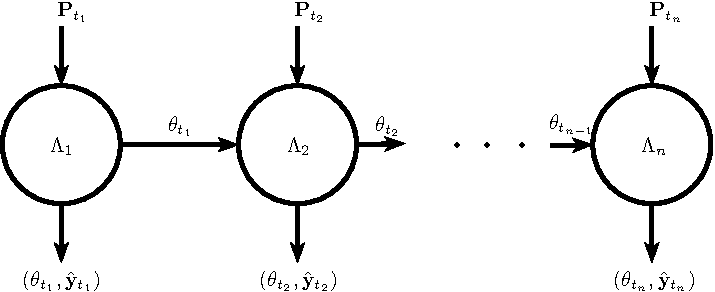
\includegraphics[clip=true,scale=0.8]{./Graphics/Lots_of_circles_3.pdf}
	\caption{\footnotesize Structure of the partial observations model with communication}
	\label{fig:PODLM}
	\end{figure}
	 
	 
	However, communication between models $\Lambda_{k-1}$ and $\Lambda_k$ may not improve the overall accuracy for every partial observations problem. For example, for a class imbalanced problem a small number of incorrect predictions in $\theta_{t_{k-1}}$ can have an adverse effect for the model $\Lambda_k$. Therefore, for some instances such as class imbalanced datasets it is desirable to have  models $\Lambda_k$ without communication between the models as shown in Figure \ref{fig:PODLM2}.  
	
	
	\begin{figure}[H]
	\centering
	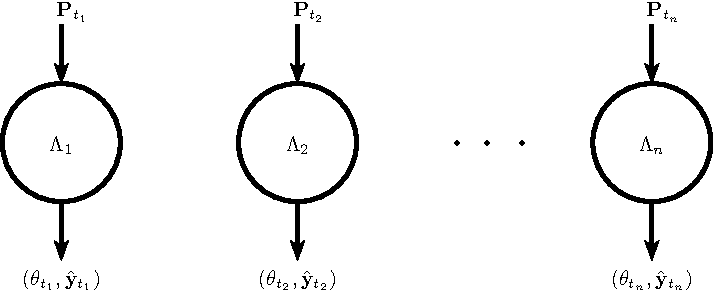
\includegraphics[clip=true,scale=0.8]{./Graphics/Lots_of_circles_4.pdf}
	\caption{\footnotesize Structure of the partial observations model without communication}
	\label{fig:PODLM2}
	\end{figure}
	
	We use developing-events classifiers and  cascaded state space models to classify events in synthetic and real-world data streams. 

	% =======================================================================
	\section{Applications} \label{sec:Experiments}
	% =======================================================================
	The R code applicable to this section is available in the supplementary material.
	\subsection{Synthetic data}\label{subsec:Synthetic}
	\subsubsection{Description}
 	The synthetic data used in this section can be generated from the R package {\it eventstream}. The synthetic data contains events of two classes: A and B. All events belonging to class A look similar, that is they have one single non-standard shape or visual pattern. In contrast, events belonging to class B  can have one of three different non-standard shapes, including the shape of events of class-A. The use of three different shapes for class B events and one shape for class A events with that shape being common with those of class B was motivated from the real-world application. 
 	
 	The Figure \ref{fig:Classes_A_And_B} illustrates the events of classes A and B.  Figure \ref{fig:Class_A} contains two events of class A, and Figure \ref{fig:Class_B} contains 3 events of class B. The shapes are labelled as $1$, $2$ or $3$ in both Figures \ref{fig:Class_A} and \ref{fig:Class_B}, with shape $1$ being the common shape.
  
  	%Motivated by the real world dataset shown in Figure \ref{fig:Real_World_Data} we create a set of synthetic files which mimic some properties of the real world dataset. Each file is a $350 \times 250$ two-dimensional array of cells/pixels. Files contain events from either one or both classes, namely  A and B.
	%[trim=0.2cm 0.7cm 1.2cm 2.4cm, clip=true, width=0.48\textwidth]	
   
  
\begin{figure}[H]
	\centering
	\subfloat[][]{
		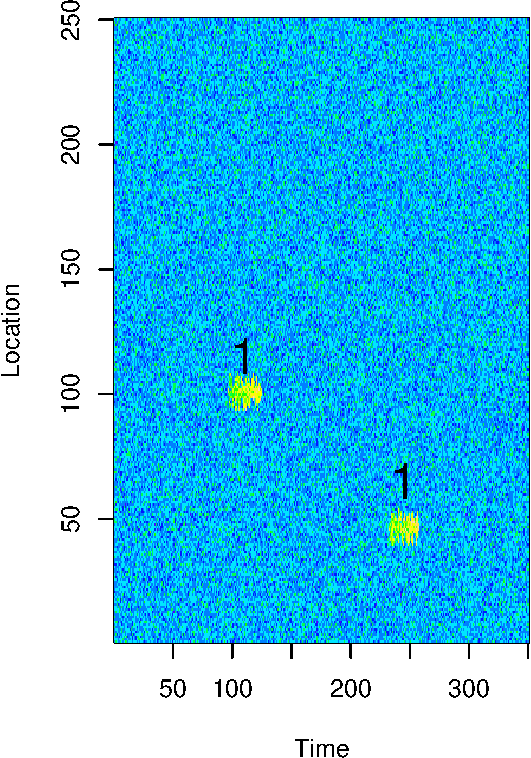
\includegraphics[clip=true, scale=0.48]{./Graphics/2_A_Blobs_labels.pdf}
		\label{fig:Class_A} % width=0.48\textwidth, height = 0.48\textheight
	}%
	\subfloat[][]{
		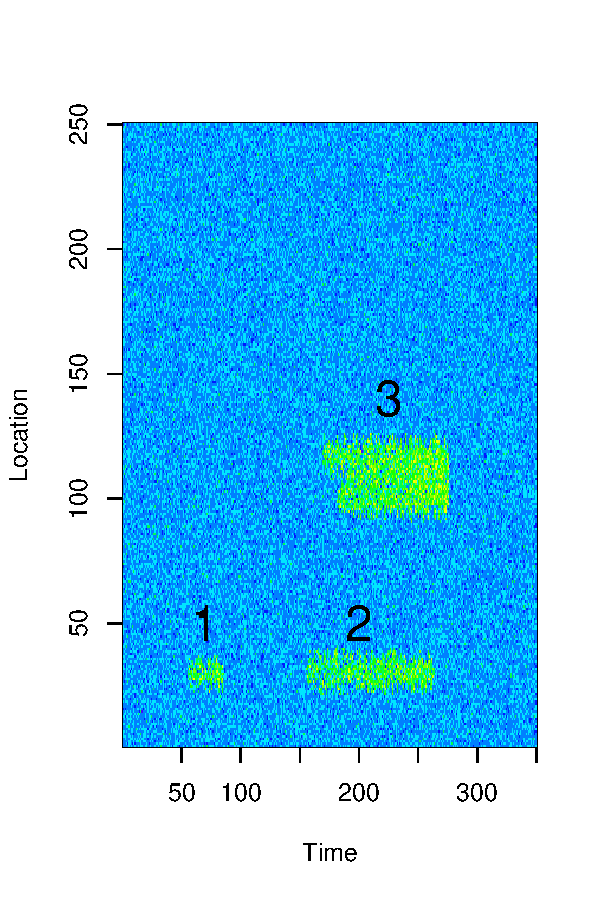
\includegraphics[clip=true, scale=0.48]{./Graphics/3_B_Blobs_labels.pdf}
		\label{fig:Class_B}
	}
	\caption{\footnotesize Class A  events in Figure \ref{fig:Class_A}  and  Class B events in Figure \ref{fig:Class_B}.  }
	\label{fig:Classes_A_And_B}
\end{figure}
	 
	The number of events of class A and B their positions are randomly generated. The other difference between the events of class A and B, apart from the shape is that values of the pixels belonging to events of class A and B come from different probability distributions. For both classes the intensity of pixel values increase linearly with the age of the event.  We list the differences between class A and B events in Table \ref{tab:DiffClassAandB}.
	
	
	\begin{table}[!ht]
		\centering
		\caption{Differences in class A and class B events. }
		\footnotesize
		\begin{tabular}{p{6cm}p{3.5cm}p{3.5cm}}
			\toprule
			Feature &  Class A value distribution & Class B value distribution \\
			\midrule
			Starting cell/pixel values     & $N(4,3)$			& $N(2, 3)$           \\
			Ending cell/pixel values       & $N(8,3)$          	& $N(4, 3)$           \\
			Maximum age of event - shape 1  & $U(20,30)$ 	    & $U(20,30)$     \\
			Maximum age of event - shape 2  & - 	 	    		& $U(100,150)$  	\\
			Maximum age of event - shape 3  & - 	 	    		& $U(100,150)$     	\\
			Maximum location width of event - shape 1  & $U(20,26)$    & $U(20,26)$       \\
			Maximum location width of event - shape 2 & -   		& $U(30,38)$  	\\
			Maximum location width of event - shape 3 & - 	 	& $U(50,58)$     	\\
			\bottomrule
		\end{tabular}
		\label{tab:DiffClassAandB}
	\end{table}
	

	 \subsubsection{Synthetic data results}
	We classify the extracted events from synthetic data using \begin{inparaenum} \item Developing-events classifier \item Cascaded state space models and \item Logistic regression.  \end{inparaenum} The R code used for all experiments is available in the supplementary material. Figure \ref{fig:TwoWindows} shows snapshots of the data and the extracted events of two successive windows.
	
	
	\begin{figure}[H]
		\centering
		\subfloat[][]{
			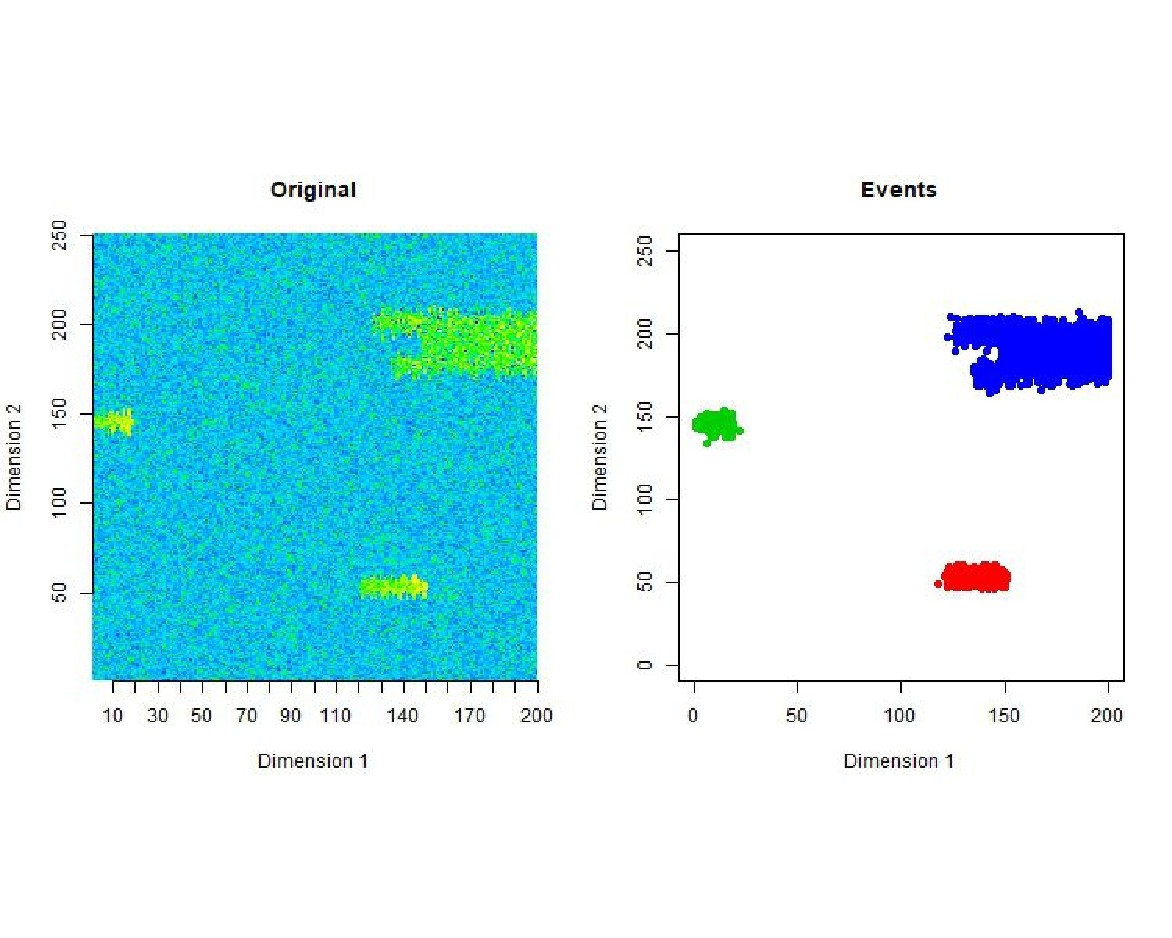
\includegraphics[clip=true, scale=0.4]{./Graphics/Events_100030.pdf}
			%\label{fig:Window_1} % width=0.48\textwidth, height = 0.48\textheight
		}%
		\subfloat[][]{
			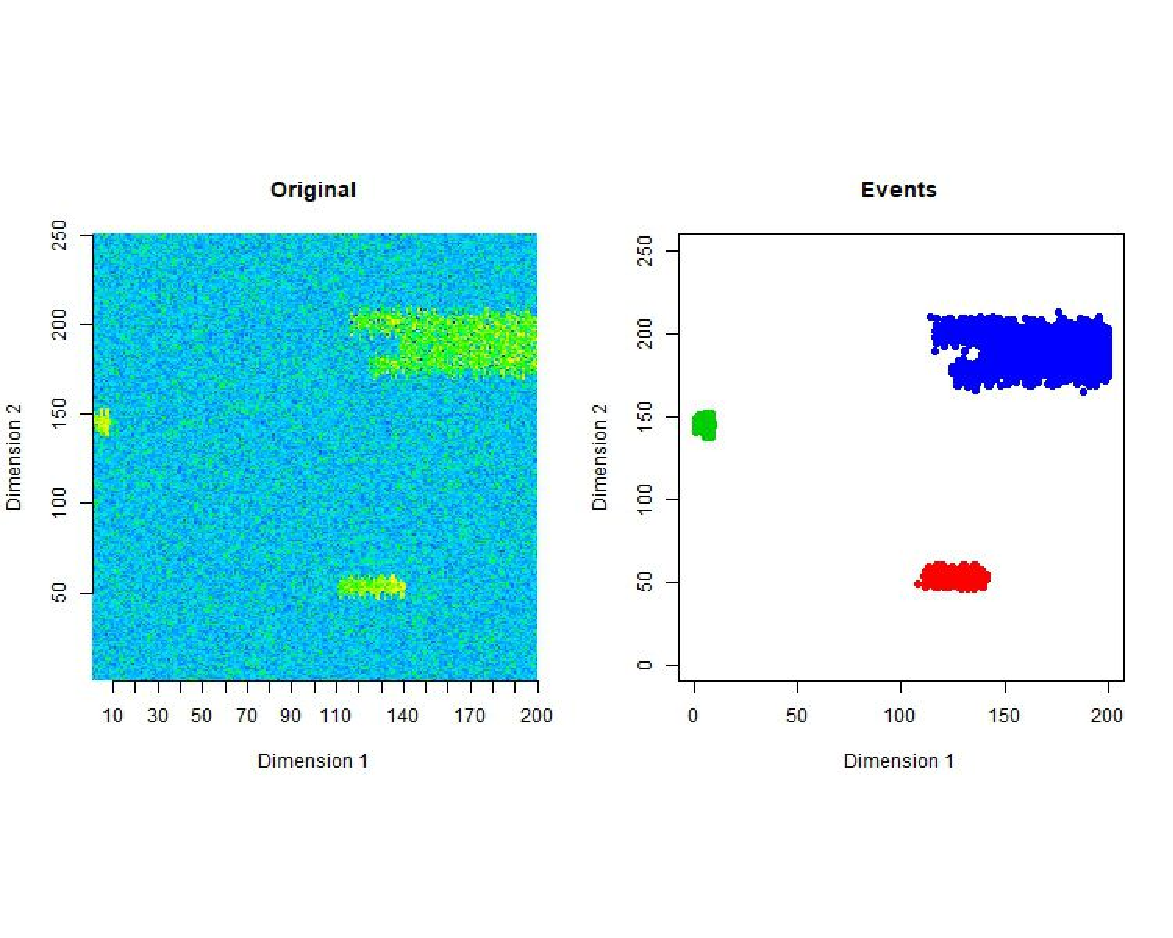
\includegraphics[clip=true, scale=0.4]{./Graphics/Events_100031.pdf}
			%\label{fig:Window_2}
		}
		\caption{\footnotesize Two successive windows of data and extracted events  }
		\label{fig:TwoWindows}
	\end{figure}
		
	
	We repeat each experiment $5$ times with data streams generated with different seeds. For each experiment we generate a data stream of dimensions $3500 \times 250 $ of which $80\%$  $(2800 \times 250 )$ is used for training and the remaining $20\%$ for testing. For  synthetic data classification, we do not use features which were motivated from the real-world example, i.e. we do not use features 11 and 12 from the list in Section \ref{sec:Featurelist}. In addition, the centroid is not used in any classification task. As class A events can have a maximum age of $30$, we use $4$ event ages for the classification tasks at  $t = 8, 16, 24$ and  $32$ time units. That is, event features are calculated at these ages.  We use a moving window model of dimensions $200 \times 250 $ which moves by a step of $ 8 \times 250$. 
	
	Figure \ref{fig:3Classifiers} shows the accuracy of the developing-events classifier, state space model and logistic regression classifier over 5 repetitions. 	From Figure \ref{fig:Facet2} we see that for each repetition either the developing-events classifier or the state space model surpasses the logistic regression classifier. From Figure  \ref{fig:Facet1} we see that the developing-events classifier performs better on average than the other two classifiers for synthetic data.  Table \ref{tab:Results_Synthetic} gives the average accuracy results for the 3 classifiers, which confirms these observations. Also we see that all 3 classifiers improve their average accuracy levels with the age of the events.
	
		
	\begin{table}[H]
		\centering
		\caption{Average accuracy $(\%)$ over $5$ repetitions }
		\footnotesize
		\begin{tabular}{p{6cm}p{1cm}p{1cm}p{1cm}p{1cm}}
			\toprule
			Classifier & Accuracy at $t_1$ & Accuracy at $t_2$  & Accuracy at $t_3$ & Accuracy at $t_4$    \\
			\midrule
			Developing-events classifier    & 81 	& 90  & 93 & 92        \\
			Cascaded state space models    & 87 	& 89  & 89 & 90        \\
			Logistic regression & 75 & 78 & 77 & 78  	\\
			\bottomrule
		\end{tabular}
		\label{tab:Results_Synthetic}
	\end{table}
	
	
	\begin{figure}[H]
	\centering
	\subfloat[][]{
		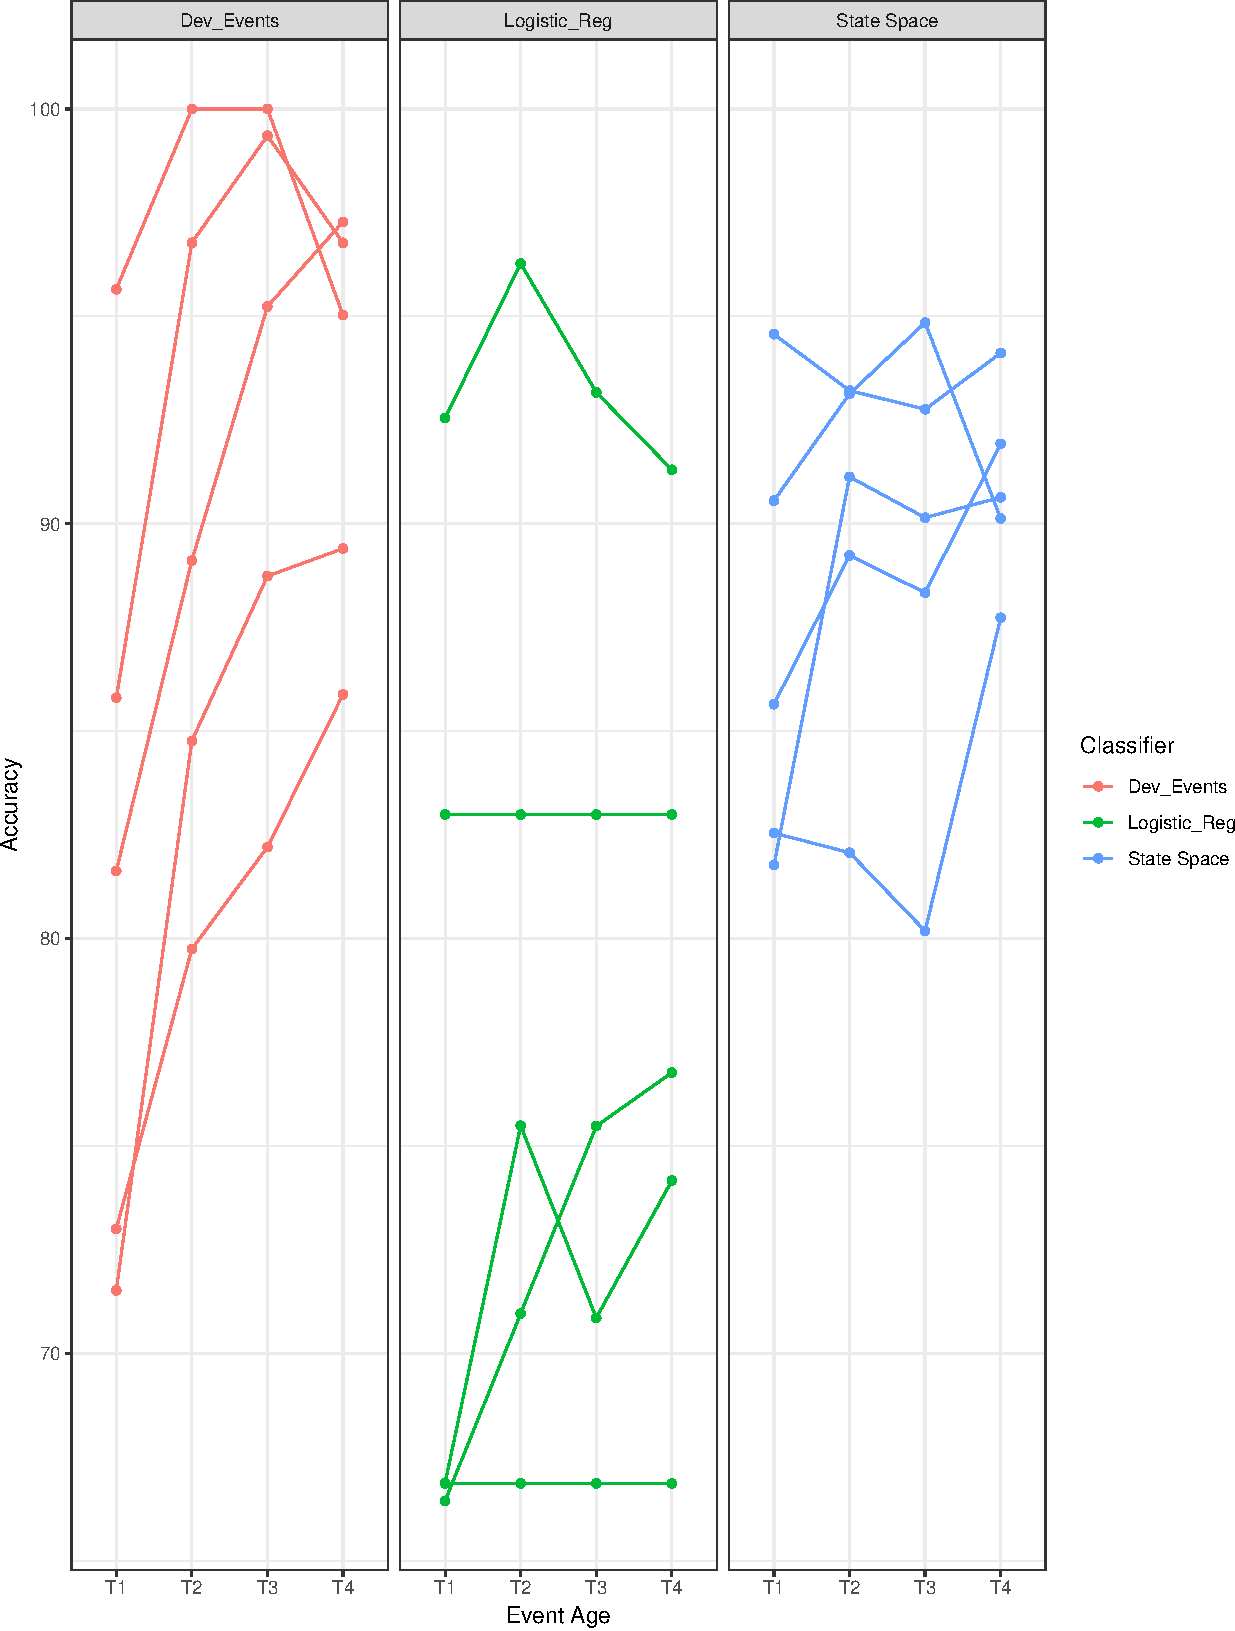
\includegraphics[clip=true, scale=0.25]{./Graphics/3_Classifiers_1.pdf}
		\label{fig:Facet1} % width=0.48\textwidth, height = 0.48\textheight
	}%
	\subfloat[][]{
		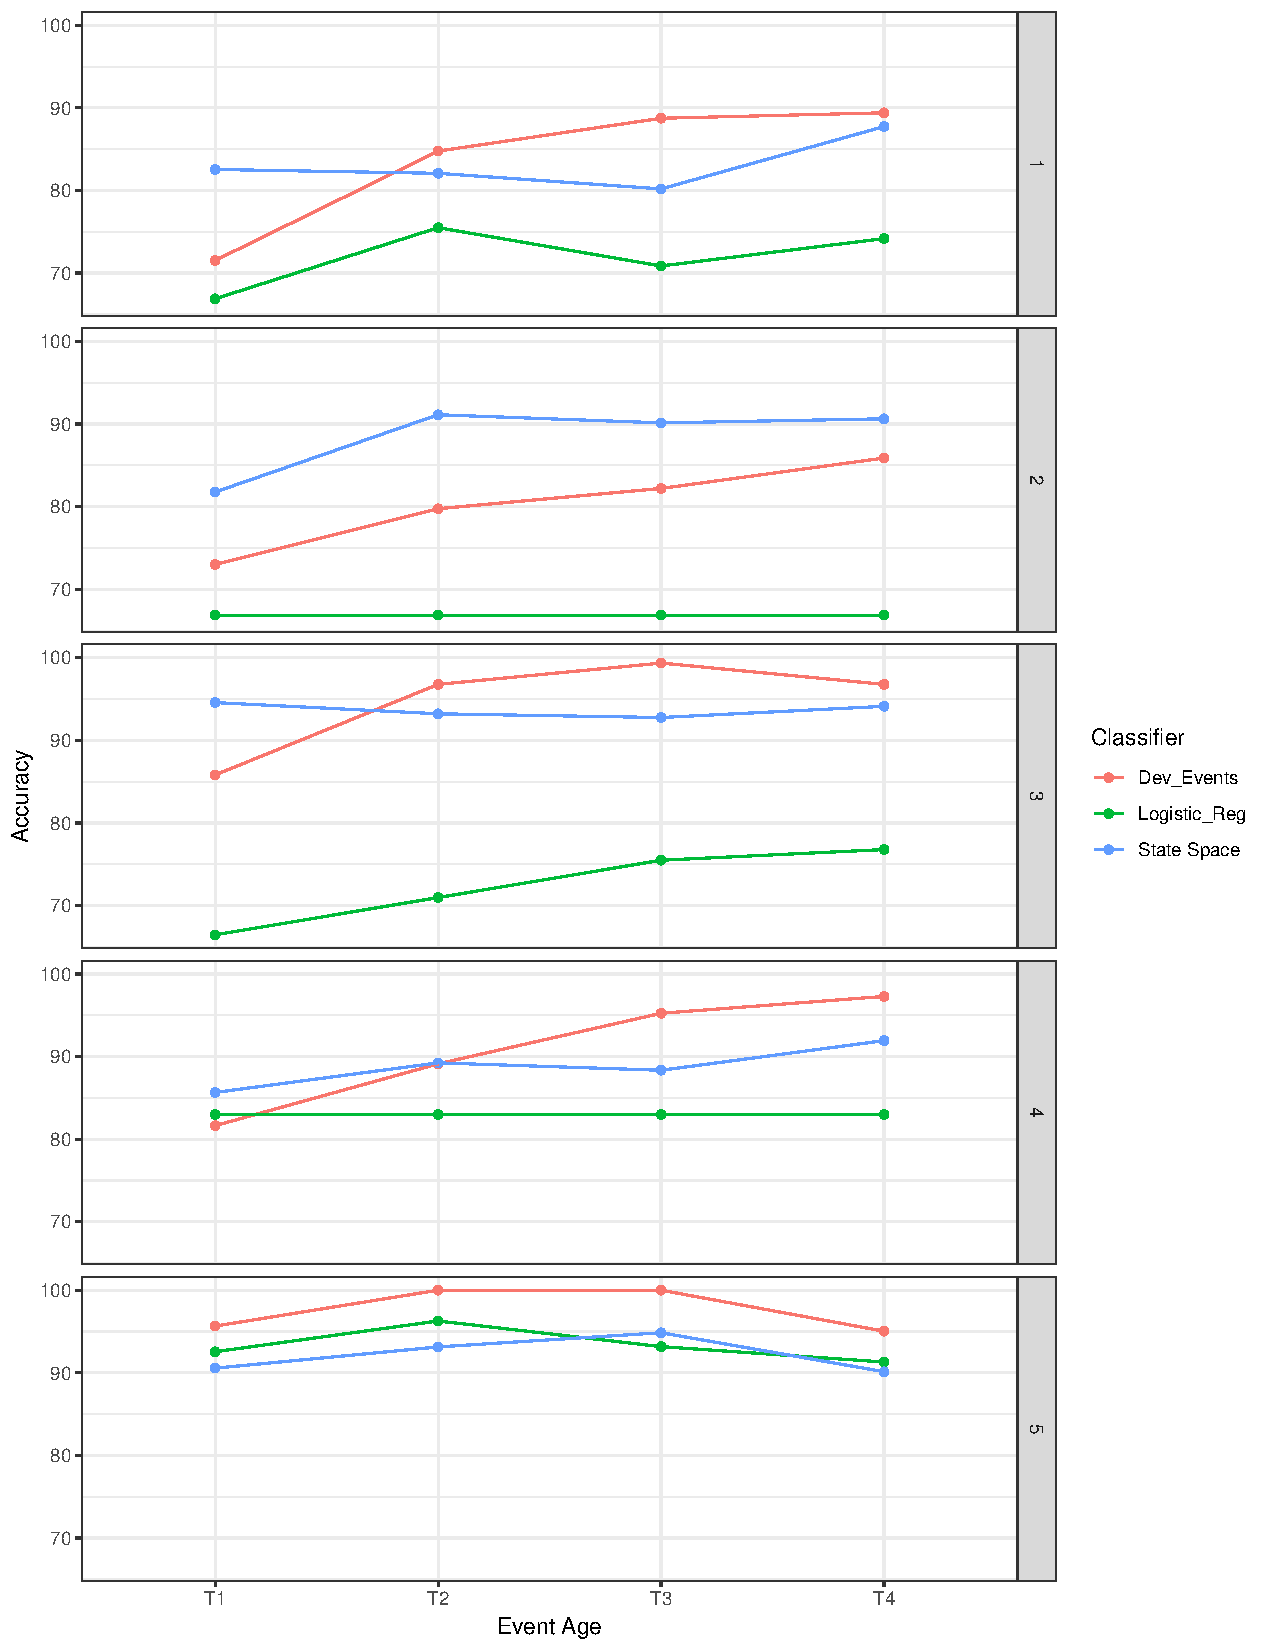
\includegraphics[clip=true, scale=0.25]{./Graphics/3_Classifiers_2.pdf}
		\label{fig:Facet2}
	}
	\caption{\footnotesize Accuracy of the 3 classifiers over 5 repeats grouped by classifier in Figure \ref{fig:Facet1}  and  by repetition in Figure \ref{fig:Facet2}. }
	\label{fig:3Classifiers}
	\end{figure}
	
    


	
	% 5 repetitions
	% glm - logistic regression
	% developing events classifier
	% cascaded dma
	% for all training 8 x 350 blocks
	% testing 2 x 350 blocks
	\subsection{Real Application 1}
	\subsubsection{Description}
 	The first real-world application is about early event classification and the associated data is available in the R package {\it eventstream}. The data stream from the real-world application is shown in Figure \ref{fig:Real_World_Data_Stream}  and has dimensions $379  \times 587 $, with class A events labelled with letter {\bf A}. The extracted events have a maximum age of 40 time units. As such, we use a window model with a window size $40 \times 587$ and a step size $ 10 \times 587$ to extract events and compute features. 
 	\begin{figure}[!ht]
 		\centering
 		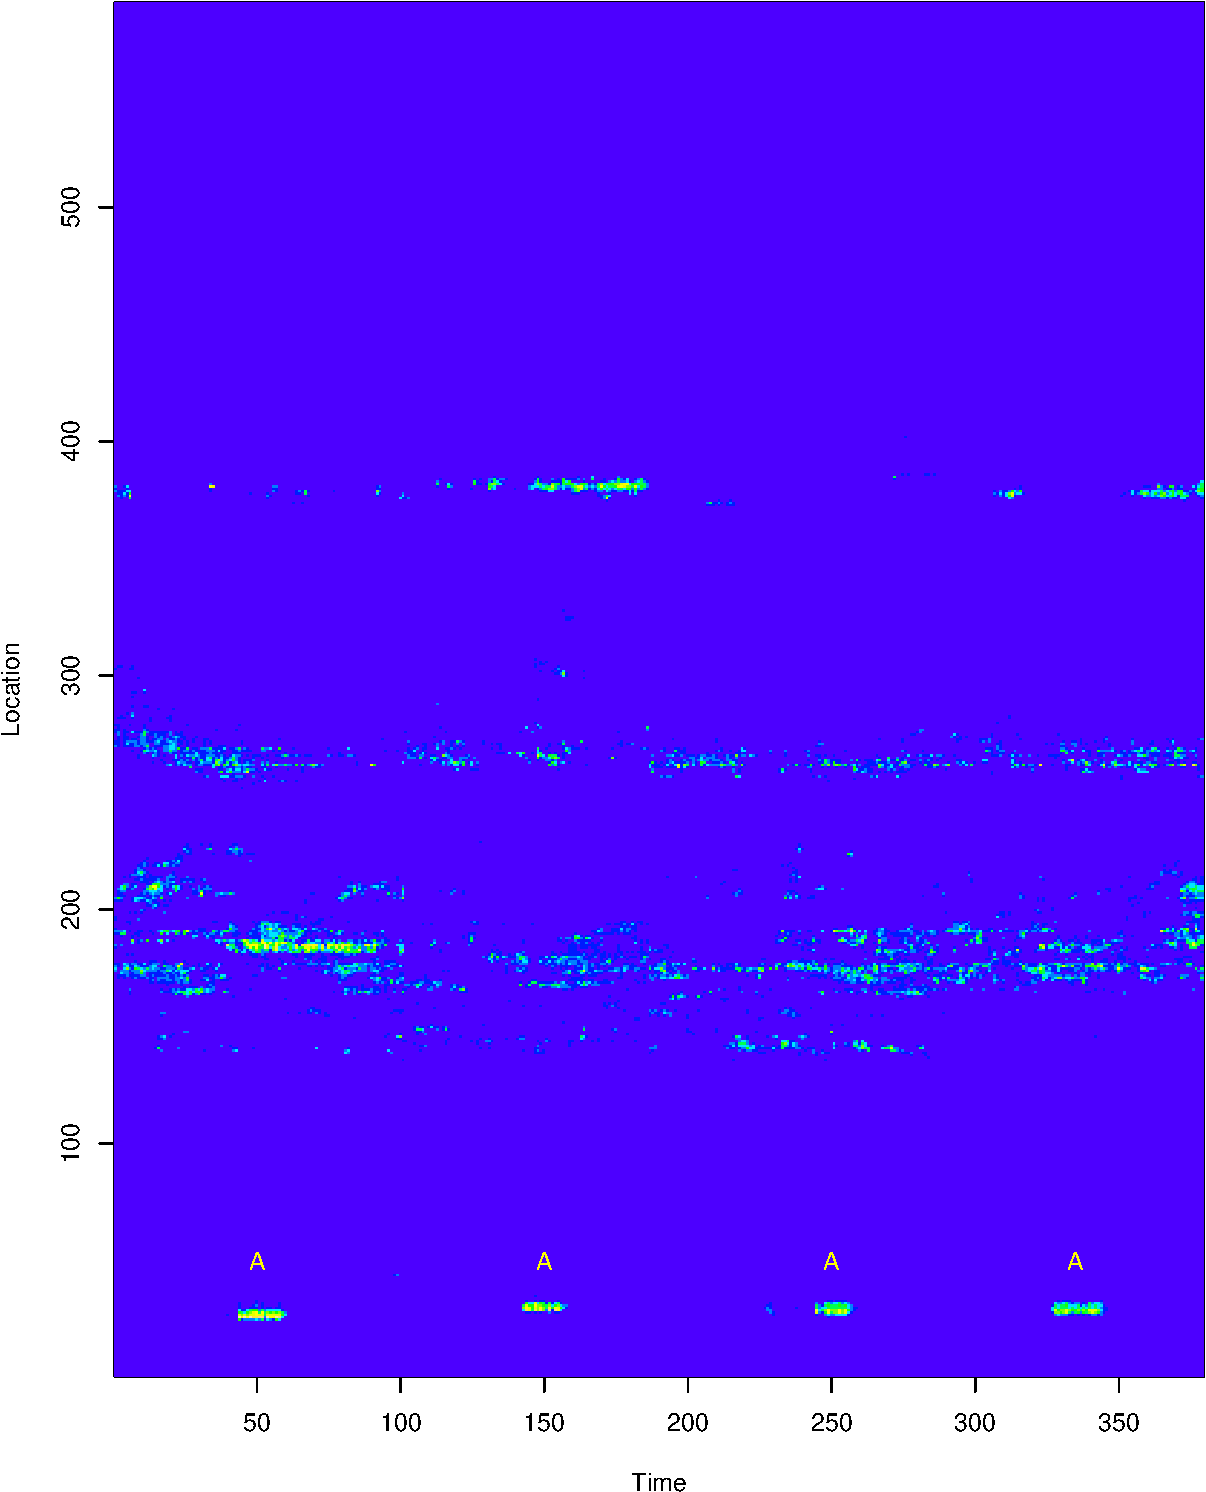
\includegraphics[scale=0.5]{./Graphics/Real_World_stream.pdf} 
 		\caption{\footnotesize Data stream from real-world application}
 		\label{fig:Real_World_Data_Stream}
 	\end{figure}
 	
 	Similar to the synthetic data stream we classify the extracted event features using 3 classifiers. The main difference is that the real data stream has a much smaller number of class A events compared to class B events.  Due of this class imbalance, we configure the state space models for real data differently from  those for synthetic data.  Firstly, we use the the state space models structure depicted in Figure \ref{fig:PODLM2} because of imbalanced classes. Secondly, as there are only $4$ class A events, there is not enough class A data to update the state space models regularly. As such we use the state space models for training and prediction without the updating step given in equation \eqref{eq:GDLM_3}. 
 	
 	
 	We use $4$-fold cross validation because there are 4 class A events, with event ages  $t = 10, 20, 30$ and  $40$, because the maximum event-age is $40$ time units. The developing-events, logistic regression and the state space models classifiers  are trained on a data stream comprising of 3 training folds, and tested on the remaining fold. 
 	
	
 	\subsubsection{Evaluation metrics}
 	We report additional accuracy measures that are geared for imbalanced datasets. These metrics are positive predictive value (PPV), negative predictive value (NPV) and area under the receiver operator characteristic curve (AUC). We give the definitions of these metrics below:
 	$$ \text{Positive predictive value (PPV)} = \frac{ \text{Number of true postives} }{ \text{Number of predicted positives}  }  \, ,   $$ 
 	
 	$$ \text{Negative predictive value (NPV)} = \frac{ \text{Number of true negatives} }{ \text{Number of predicted negatives}  }  \, ,   $$ 
 	
 	\noindent
	The number of predicted positives in PPV is the sum of true positives and false positives, and similarly the number of predicted negatives in NPV is the sum of true negatives and the false negatives. Both PPV and NPV separately gives only  one-sided accuracy measures. For example, a classifier that predicts all observations negative except for one correct positive observation achieves a PPV of $100\%$ but a small NPV. As such, the combination of PPV and NPV gives the overall accuracy of the model. 
	
	In contrast, the area under the receiver operator characteristic (ROC) curve  is a single measure that captures the effectiveness of a classifier. The ROC curve is a plot of the true positive rate against the false positive rate for different classification thresholds. The area under the curve (AUC) provides a measure of discrimination between positive and negative classes. The AUC can be interpreted as the probability that a positive observation is ranked higher than a negative observation. The AUC does not depend on the classification threshold as it is an aggregate measure.  An AUC closer to 1 is reflective of a good model, while a random predictor will give an AUC closer to 0.5. 
	

	\subsubsection{Real data results}
	The graphs in Figures \ref{fig:RealPPV}, \ref{fig:RealNPV} and \ref{fig:RealROC} give the PPV, NPV and AUC values of the 3 classifiers grouped by classifier and fold. Table \ref{tab:AverageAccuracyReal} gives the average PPV, NPV and AUC values over the $4$-folds for the real data stream.
	
	% PPV - dev events 0.964285714	1	1	0.964285714
	% PPV - dma 0.683333333	0.816071429	0.85625	0.6375
	% PPV - glm 0.792857143	0.673809524	0.673809524	0.721428571
	
	
	% NPV - dev events 0.930591631	0.947510823	0.936273449	0.902435065
	% NPV - dma 0.978968254	1	0.986842105	0.992647059
	% NPV - glm 0.953860029	0.965097403	0.959541847	0.965891053
	
	% AUC - dev events 0.947438672	0.973755411	0.968136724	0.93336039
	% AUC - dma 0.874206349	0.985603408	0.902065826	0.943148926
	% AUC - glm 0.873358586	0.819453463	0.816675685	0.843659812
	

	
	
	\begin{figure}[H]%[!ht]%
		\centering
		\subfloat[][]{
			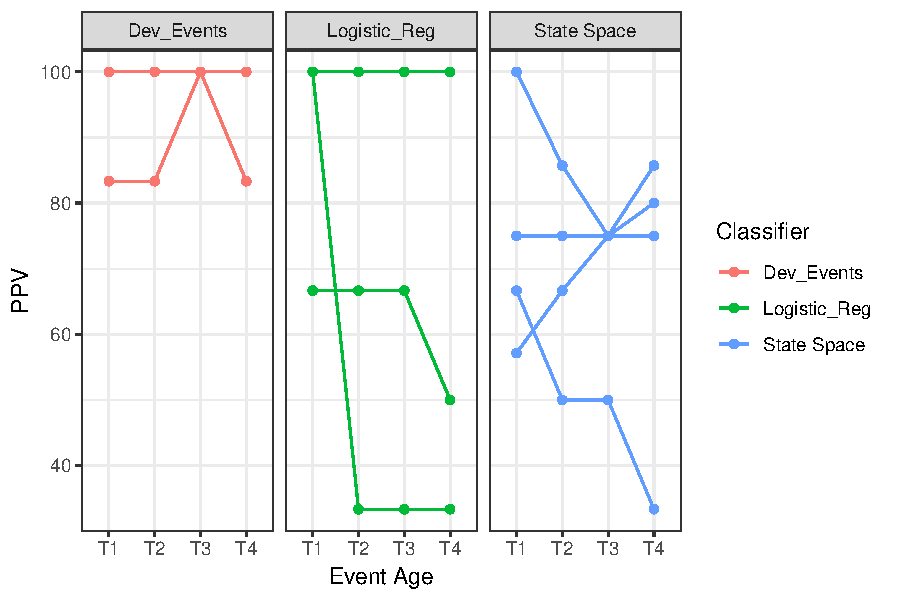
\includegraphics[clip=true, scale=0.5]{./Graphics/Real_World_PPV_1.pdf}
			\label{fig:PPV1} % width=0.48\textwidth, height = 0.48\textheight
		}%
		\subfloat[][]{
			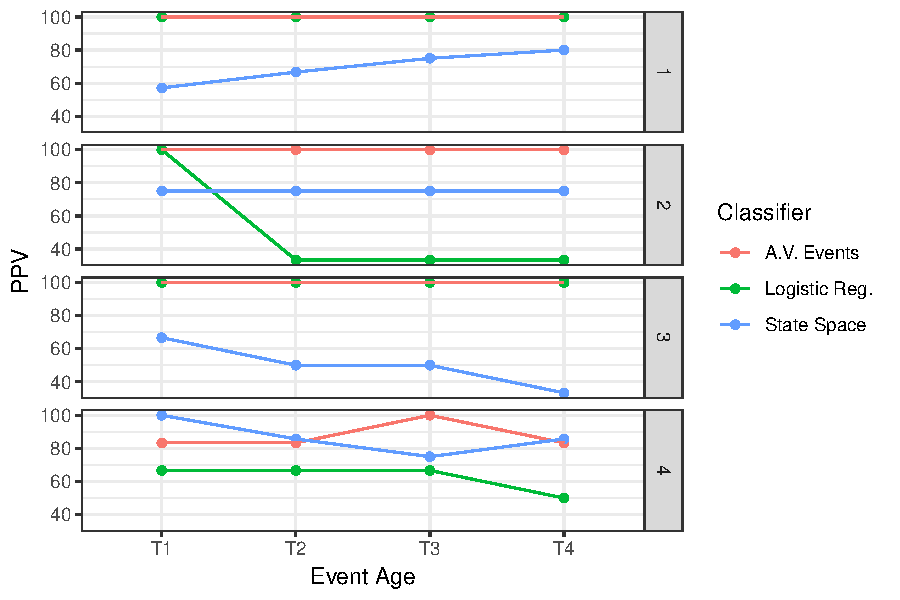
\includegraphics[clip=true, scale=0.5]{./Graphics/Real_World_PPV_2.pdf}
			\label{fig:PPV2}
		}
		\caption{\footnotesize PPV of the 3 classifiers with 4-fold cross validation grouped by classifier in Figure \ref{fig:PPV1}  and  by fold in Figure \ref{fig:PPV2}. }
		\label{fig:RealPPV}
	\end{figure}
	
	
	\begin{figure}[H]%[!ht]%
		\centering
		\subfloat[][]{
			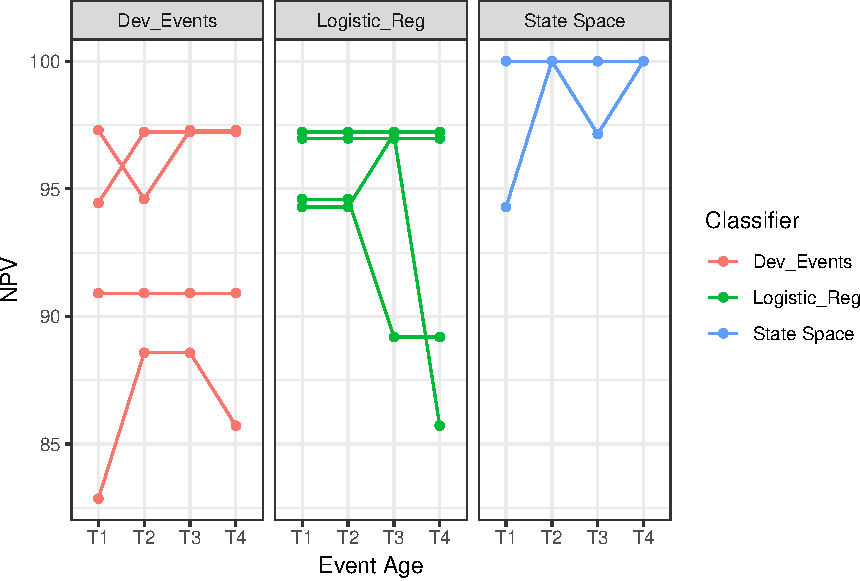
\includegraphics[clip=true, scale=0.5]{./Graphics/Real_World_NPV_1.pdf}
			\label{fig:NPV1} % width=0.48\textwidth, height = 0.48\textheight
		}%
		\subfloat[][]{
			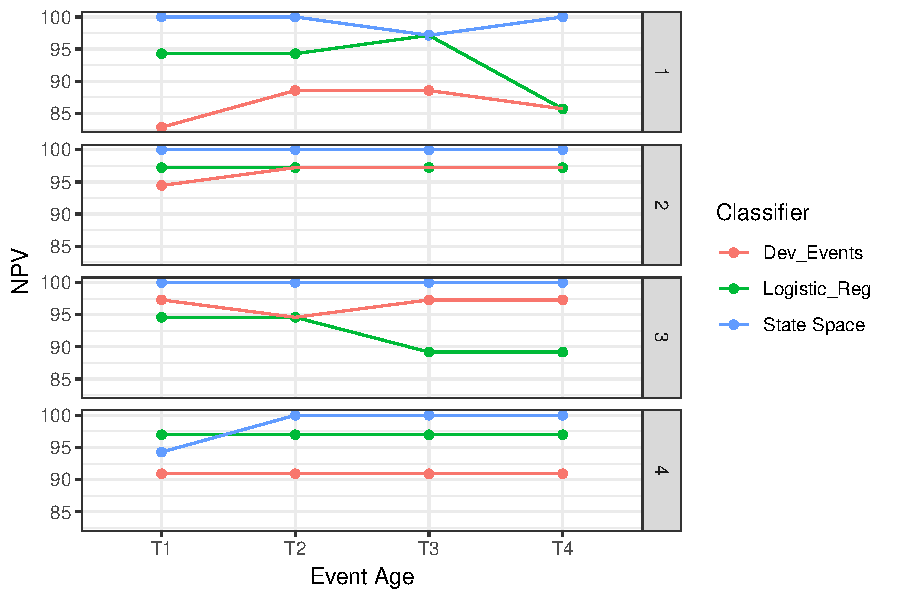
\includegraphics[clip=true, scale=0.5]{./Graphics/Real_World_NPV_2.pdf}
			\label{fig:NPV2}
		}
		\caption{\footnotesize NPV of the 3 classifiers with 4-fold cross validation grouped by classifier in Figure \ref{fig:NPV1}  and  by fold in Figure \ref{fig:NPV2}. }
		\label{fig:RealNPV}
	\end{figure}


	\begin{figure}[H]%[!ht]%
		\centering
		\subfloat[][]{
			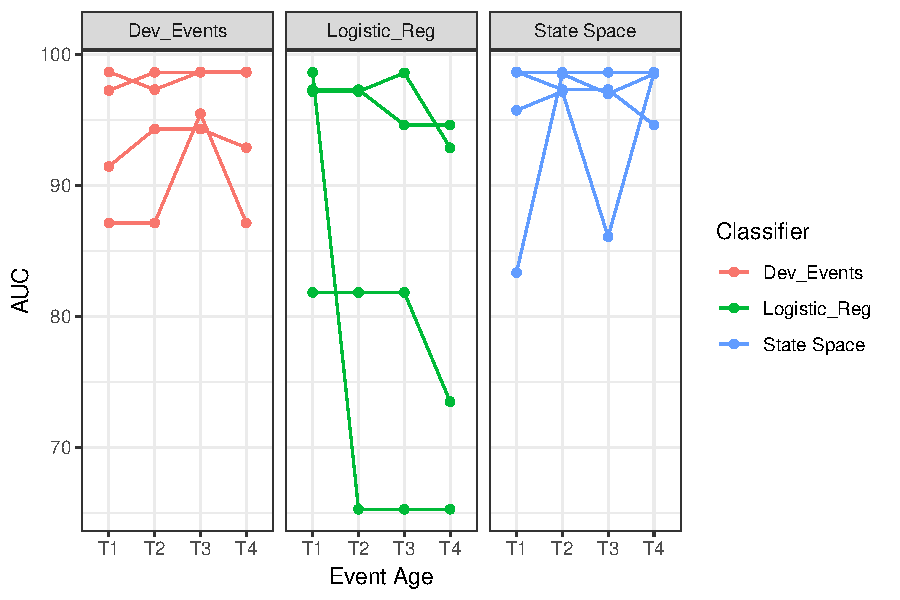
\includegraphics[clip=true, scale=0.5]{./Graphics/Real_World_ROC_1.pdf}
			\label{fig:ROC1} % width=0.48\textwidth, height = 0.48\textheight
		}%
		\subfloat[][]{
			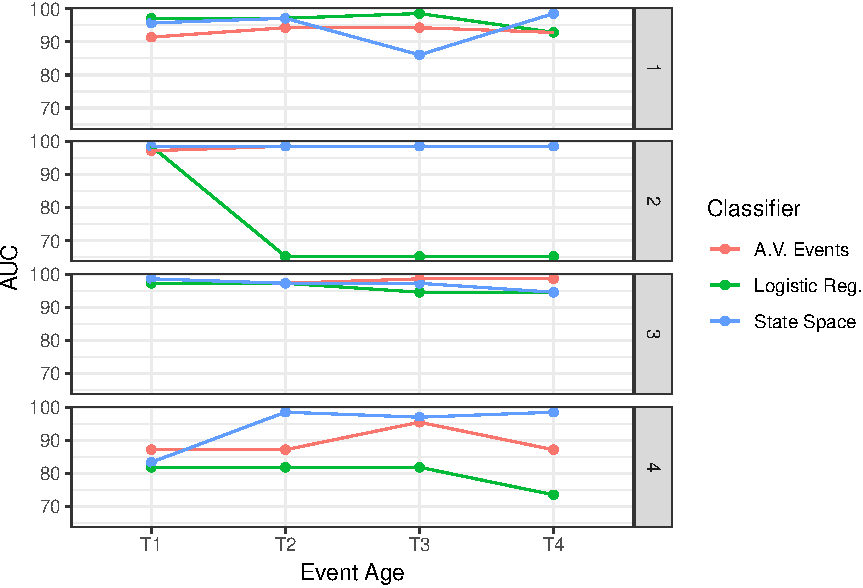
\includegraphics[clip=true, scale=0.5]{./Graphics/Real_World_ROC_2.pdf}
			\label{fig:ROC2}
		}
		\caption{\footnotesize AUC of the 3 classifiers with 4-fold cross validation grouped by classifier in Figure \ref{fig:ROC1}  and  by fold in Figure \ref{fig:ROC2}. }
		\label{fig:RealROC}
	\end{figure}
	
	\begin{table}[H]
		\centering
		\caption{Average PPV, NPV and AUC $(\%)$ over $4$ folds }
		\footnotesize
		\begin{tabular}{p{1.5cm}p{6cm}p{1cm}p{1cm}p{1cm}p{1cm}}
			\toprule
			Accuracy Measure & Classifier & At $t_1$ & At $t_2$  & At $t_3$ & At $t_4$    \\
			\midrule
			PPV & 	Developing-events classifier    & 95 	& 95  & 100 & 95        \\
			& Cascaded state space models    &74 	& 69  & 68 & 68        \\
			& Logistic regression & 91 & 75 & 75 & 70  	\\
			\hline	
			NPV & 	Developing-events classifier    & 91 	& 92  & 93 & 92        \\
			& Cascaded state space models    & 98 	& 100  & 99 & 100        \\
			& Logistic regression & 95 & 95 & 95 & 92  	\\
			\hline	  	
			AUC & 	Developing-events classifier    & 93 	& 94  & 96 & 94        \\
			& Cascaded state space models    & 94 	& 97  & 94 & 97        \\
			& Logistic regression & 93 & 85 & 85 & 81  	\\
			\bottomrule
		\end{tabular}
		\label{tab:AverageAccuracyReal}
	\end{table}

	From Table \ref{tab:AverageAccuracyReal} we see that the developing-events classifier has the highest average PPV and the cascaded state space models have the highest average NPV for all event ages. In terms of AUC both the developing-events classifier and the state space models out perform the logistic regression classifier.
	
	
	\subsection{Real Application 2}
	\subsubsection{Description}
	The second real-world application focusses on event extraction from Nitrogen Dioxide $(\text{NO}_2)$ data from NASA's NEO website \cite{OMINO2}. The Ozone Monitoring Instrument (OMI) \cite{levelt2006ozone} aboard the Aura satellite records a variety of air quality measures including $\text{NO}_2$ concentrations around the world. We use some of this data to demonstrate the event extraction and feature computation process for a 3-dimensional data stream.
	
	We use OMI $\text{NO}_2$ monthly data from March to June in the years 2008 and 2018 for a comparison study. For each month the data comes in a matrix of $1799 \times 3600 $ dimensions. For ease of calculation we reduce the dimension of this matrix to $180 \times 360 $, by computing the average of each $10 \times 10$ block of data in the original matrix. The OMI $\text{NO}_2$ March 2008 data is shown in Figure \ref{fig:NO2March2008}. 

	\begin{figure}[H]
		\centering
		\subfloat[][]{
			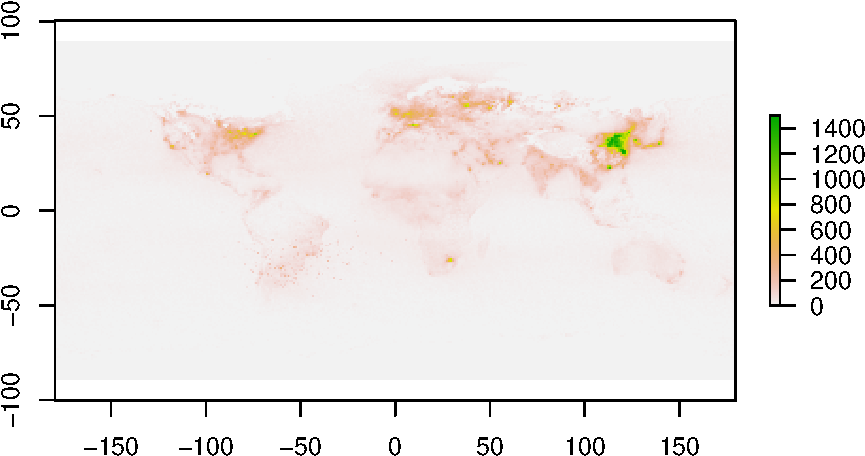
\includegraphics[clip=true, scale=0.5]{./Graphics/NO2_March_2008_No_Bndry.pdf}
			\label{fig:NO2March1} % width=0.48\textwidth, height = 0.48\textheight
		}%
		\subfloat[][]{
			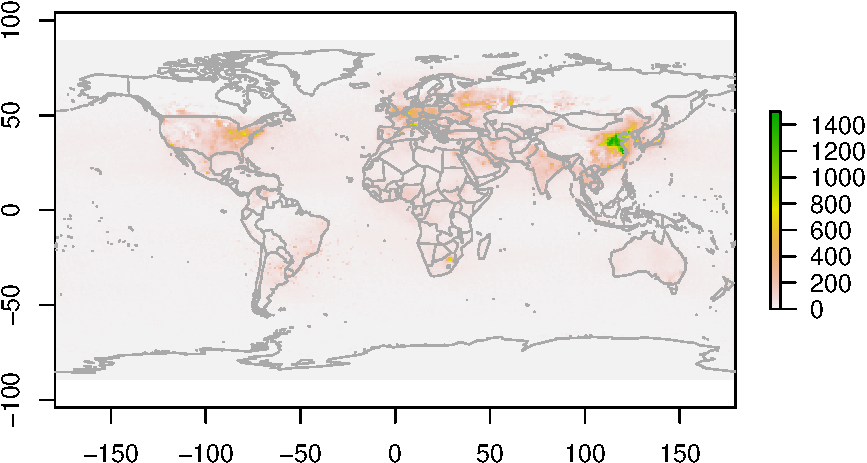
\includegraphics[clip=true, scale=0.5]{./Graphics/NO2_March_2008_With_Bndry.pdf}
			\label{fig:NO2March2}
		}
		\caption{\footnotesize $\text{NO}_2$ data for March 2008, without the world map super-imposed in Figure \ref{fig:NO2March1}, with the world map in Figure \ref{fig:NO2March2} }
		\label{fig:NO2March2008}
	\end{figure}

	
	\subsubsection{Event extraction}
	 Using Algorithm \ref{algo:events_extraction}, we extract events from this data, which are clusters of high  $\text{NO}_2$ levels spanning in space and time.  Events are extracted from a 3-dimensional data stream of $4 \times 180 \times 360$ array, where each $180 \times 360$ matrix corresponds to the $\text{NO}_2$ levels of a given month. Figure \ref{fig:ClustersNO2March2008} shows these clusters at a single snapshot of time, i.e. in March 2008. The parameters used in Algorithm \ref{algo:events_extraction} are $\alpha = 0.97$, $\epsilon=2$ and $\text{minPts} = 20$. There are 23 events/clusters in 2008 data and 13 events/clusters in 2018 data. Each event is depicted by a single colour in Figures \ref{fig:ClustersNO2March2008} and \ref{fig:ClustersNO2March2018}. 
	
	\begin{figure}[H]
		\centering
		\subfloat[][]{
			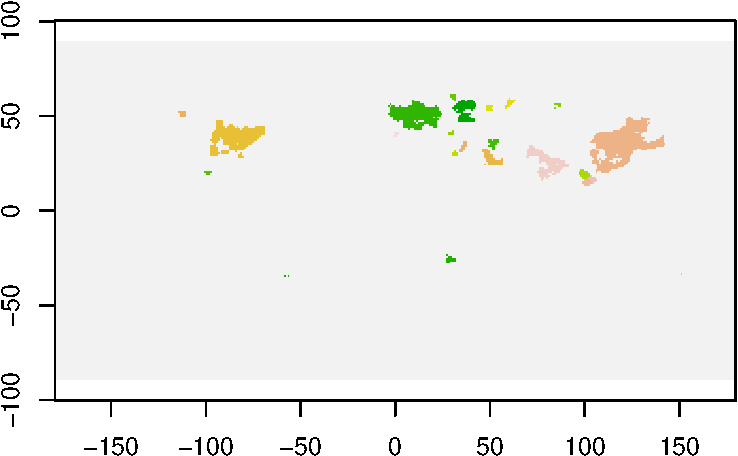
\includegraphics[clip=true, scale=0.5]{./Graphics/Clusters_NO2_March_2008_No_Bndry.pdf}
			\label{fig:ClustersNO2March20081} % width=0.48\textwidth, height = 0.48\textheight
		}%
		\subfloat[][]{
			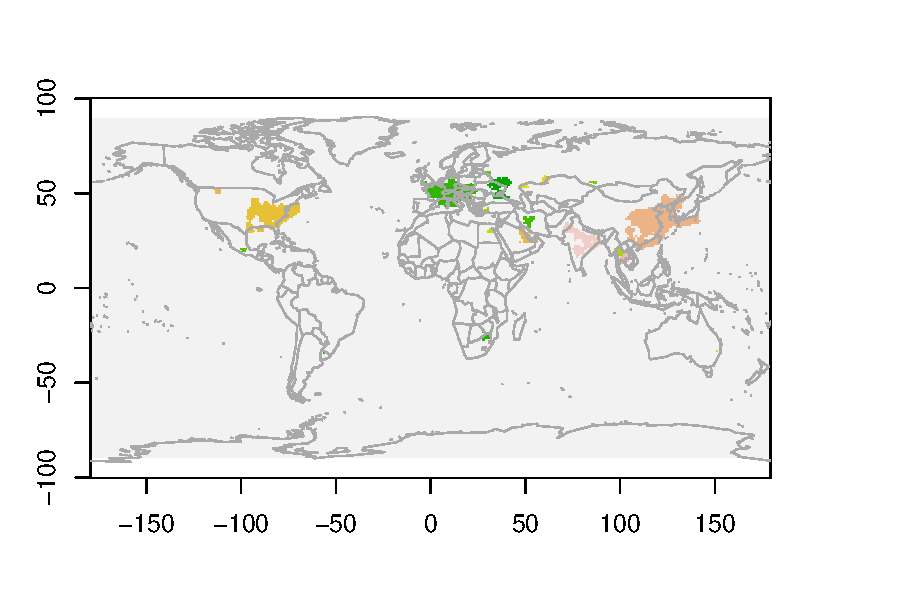
\includegraphics[clip=true, scale=0.5]{./Graphics/Clusters_NO2_March_2008_With_Bndry.pdf}
			\label{fig:ClustersNO2March20082}
		}
		\caption{\footnotesize Events extracted from $\text{NO}_2$ data for 2008. Both figures show events at a single snapshot of time in March 2008. Figure \ref{fig:ClustersNO2March20081} shows these events without the world map super-imposed and Figure \ref{fig:ClustersNO2March20082}  with the world map. Colours do not reflect $\text{NO}_2$ levels.  }
		\label{fig:ClustersNO2March2008}
	\end{figure}
	
	
	\begin{figure}[H]
		\centering
		\subfloat[][]{
			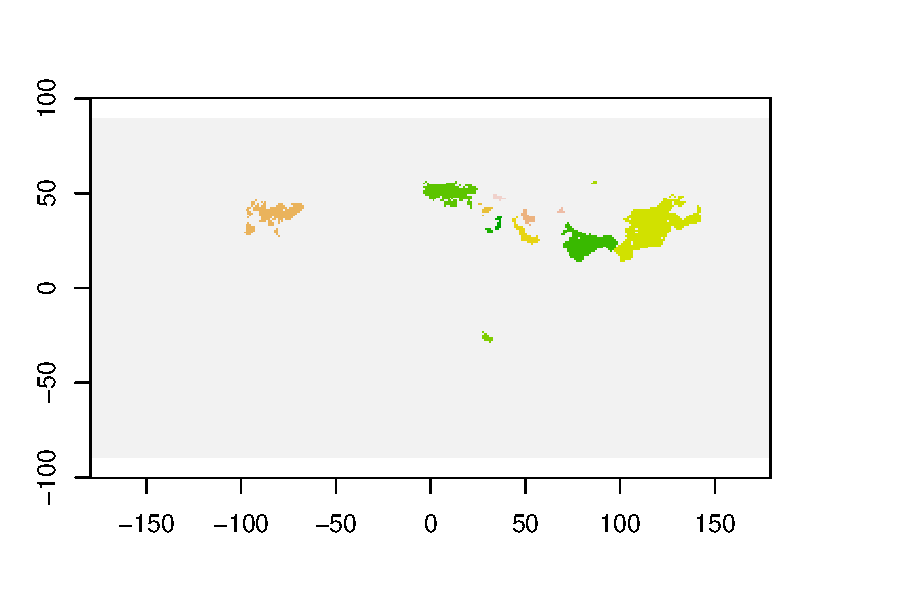
\includegraphics[clip=true, scale=0.5]{./Graphics/Clusters_NO2_March_2018_No_Bndry.pdf}
			\label{fig:ClustersNO2March20181} % width=0.48\textwidth, height = 0.48\textheight
		}%
		\subfloat[][]{
			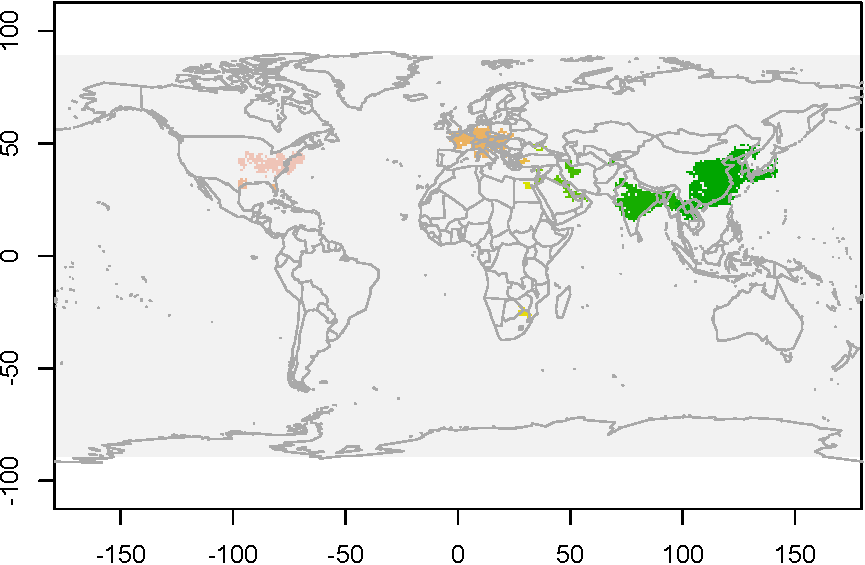
\includegraphics[clip=true, scale=0.5]{./Graphics/Clusters_NO2_March_2018_With_Bndry.pdf}
			\label{fig:ClustersNO2March20182}
		}
		\caption{\footnotesize Events extracted from $\text{NO}_2$ data for 2018. Both figures show events at a single snapshot of time in March 2018. Figure \ref{fig:ClustersNO2March20181} shows these events without the world map super-imposed and Figure \ref{fig:ClustersNO2March20182}  with the world map. Colours do not reflect $\text{NO}_2$ levels.}
		\label{fig:ClustersNO2March2018}
	\end{figure}
	

	
	\subsubsection{Event analysis}
	
	For each event we compute features 1 - 8 and 11 from the list of features in  Section \ref{sec:Featurelist}. We analyse the event which has the highest average $\text{NO}_2$ levels for 2008 and 2018. The map in Figure \ref{fig:HighestEventNO2200820181} shows the event location in March 2018 and the graph in  Figure \ref{fig:HighestEventNO2200820182} shows that the average  $\text{NO}_2$ levels have decreased in 2018 compared to 2008 for this event.


	\begin{figure}[H]
	\centering
	\subfloat[][]{
		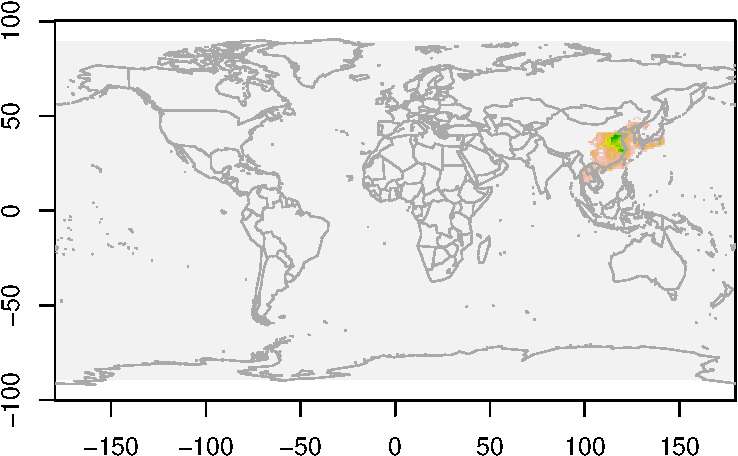
\includegraphics[clip=true, scale=0.5]{./Graphics/High_Event_2018.pdf}
		\label{fig:HighestEventNO2200820181} 
	}%
	\subfloat[][]{
		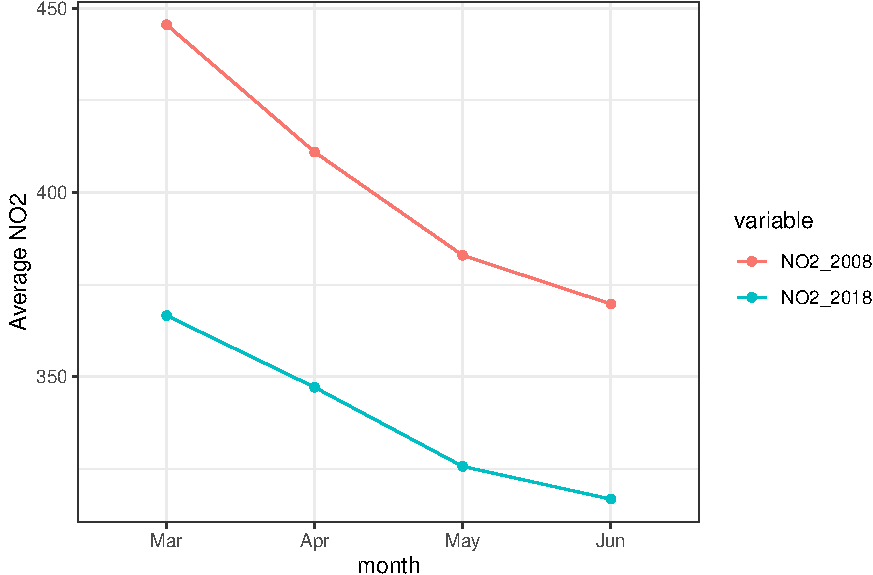
\includegraphics[clip=true, scale=0.4]{./Graphics/Highest_Event_NO2_2008_2018.pdf}
		\label{fig:HighestEventNO2200820182}
	}
	\caption{\footnotesize The location of the event with the highest average $\text{NO}_2$ levels in Figure \ref{fig:HighestEventNO2200820181}, and the associated $\text{NO}_2$ in 2008 and 2018 in Figure \ref{fig:HighestEventNO2200820182}. }
	\label{fig:HighestEventNO220082018}
	\end{figure}
	
	
	Next we match the events in 2008 and 2018 by their spatial location. We do a simple analysis of these $\text{NO}_2$ events. We want to know if these  $\text{NO}_2$ events have increased or decreased in severity during this 10 year time gap. 

	
	For each of these matched events we find the  average $\text{NO}_2$ level difference between 2018 and 2008. The Figure \ref{fig:DifferenceInNO2Levels} shows the graph of these differences. 
	
	\begin{figure}[H]
		\centering
		\subfloat[][]{
			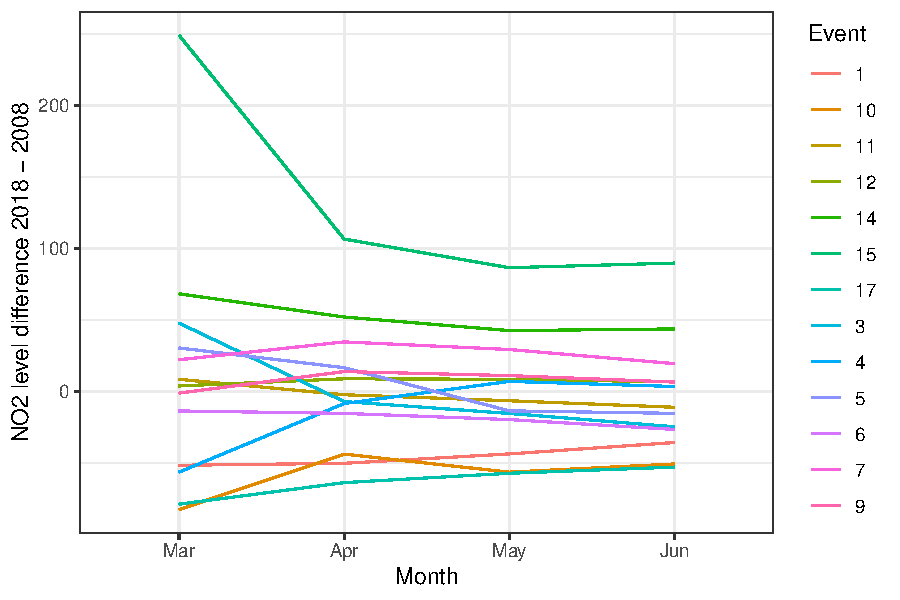
\includegraphics[clip=true, scale=0.5]{./Graphics//NO2_Level_Difference_2018_2008.pdf}
			\label{fig:DifferenceInNO2Levels1} 
		}%
		\subfloat[][]{
			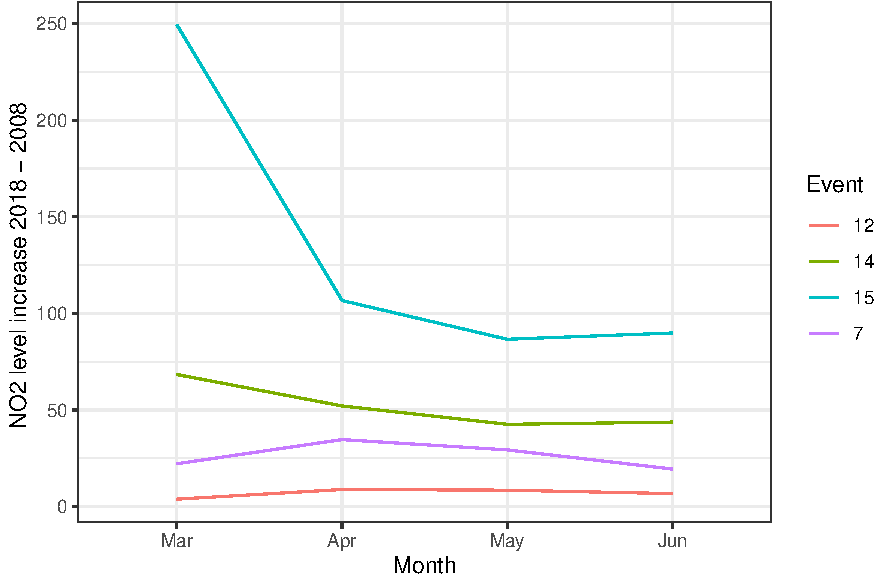
\includegraphics[clip=true, scale=0.5]{./Graphics/NO2_Level_Increase_2018_2008.pdf}
			\label{fig:DifferenceInNO2Levels2}
		}
		\caption{\footnotesize Difference in average  $\text{NO}_2$ levels; 2018 - 2008 in Figure \ref{fig:DifferenceInNO2Levels1} for all matched events. The events for which average $\text{NO}_2$ level difference is positive, i.e. average $\text{NO}_2$ levels have increased from 2008 to 2018, in Figure \ref{fig:DifferenceInNO2Levels2}.}
		\label{fig:DifferenceInNO2Levels}
	\end{figure}
	
	From Figure \ref{fig:DifferenceInNO2Levels} we see that 4 events have positive $\text{NO}_2$ differences for each month, i.e. the average $\text{NO}_2$ levels have increased from 2008 to 2018 for these 4 events. In addition event 15 is different from other events. Figure \ref{fig:PositiveDifferentEventsNO220082018} shows the  locations of the increased $\text{NO}_2$ events in March 2018 along with the  location of the outlying event 15. 
	 	
	\begin{figure}[H]
		\centering
		\subfloat[][]{
			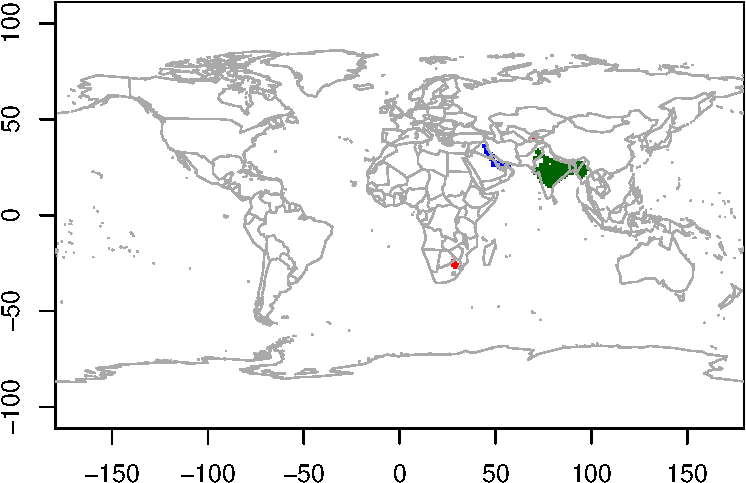
\includegraphics[clip=true, scale=0.5]{./Graphics/Positive_NO2_Events_2018_2008.pdf}
			\label{fig:PositiveEventNO220082018} 
		}%
		\subfloat[][]{
			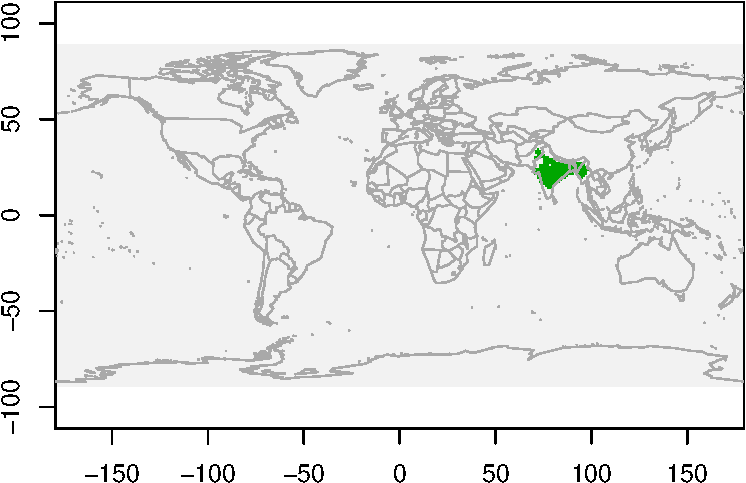
\includegraphics[clip=true, scale=0.5]{./Graphics/Different_Event_2018_2008.pdf}
			\label{fig:DifferentEventNO220082018}
		}
		\caption{\footnotesize The location in March 2018 of events with increased  average $\text{NO}_2$ levels in Figure \ref{fig:PositiveEventNO220082018}, and the outlying $\text{NO}_2$ event in Figure \ref{fig:DifferentEventNO220082018}. }
		\label{fig:PositiveDifferentEventsNO220082018}
	\end{figure}

	While the increased industrialization in India and the ongoing war in the Middle-East regions may be contributors, an investigation of reasons behind the increased $\text{NO}_2$ levels is beyond the scope of this study. Our aim is to demonstrate the applicability of our event extraction and event classification algorithms for different applications. We re-state that the code for this analysis is available in the supplementary material.
		
	% =======================================================================
	\section{Conclusions}\label{sec:Conclusions}
	% =======================================================================
	
	This paper investigates a framework for event extraction and early event classification in data streams with a focus on early event classification. We focus on time-varying coefficient models for event classification.  To this end we propose two classifiers; a static and an updating classifier, both of which take developing event features/partial observations as input. We test our framework using 3 applications; one synthetic data application and two real-world applications. We show that we obtain better accuracy results compared to logistic regression for these applications. 
	
	In addition, we propose an algorithm for event extraction, which can be used on two or three dimensional data streams. We show the applicability of our event extraction algorithm using the $\text{NO}_2$ data from NASA's NEO website.    
	Future directions of research include extending the developing-events classifier to have an automatically updating coefficients and including a variety of  event extraction processes.      
	
	% =======================================================================
	\section*{Acknowledgements}
	% =======================================================================
	Funding was provided by the Australian Research Council through the Linkage Project LP160101885. The first author would like to thank Dr Andres Ramirez Hassan for useful discussions.
	
	\footnotesize
	\bibliographystyle{IEEEtran} %Choose a bibliograhpic style
	\bibliography{Master}
	
	
%1. A clustering approach for structural health monitoring on bridges \\
%2. Event Detection from Video Surveillance Data Based on Optical Flow Histogram and High-level Feature Extraction \\
% =======================================================================
\end{document}
% =======================================================================


	%% Outline
%% 1. Introduction 
%% 1.1		data streams - what is being done - literature
%% 1.2 		What they don't address
%% 1.3      What we do - a statistical approach for event classification
%% 2. Motivation & research problem 
%% 2.1 		Real world example - early detection really important
%% 3  Notation - Our partial information model	
%% 4. Partial observations classifiers
%%		- Explain the penalty and everything
%% 5. Cascaded Dynamic Linear Models for our work
%% 6. Datasets, Blob extraction, Features
%% 7  Results
%% 8. Future work and Conclusions